% !TEX TS-program = xelatex
% !TEX encoding = UTF-8

% This is a simple template for a XeLaTeX document using the "article" class,
% with the fontspec package to easily select fonts.

 % use larger type; default would be 10pt
\documentclass[10pt]{book}
\usepackage[czech]{babel}
\usepackage{ucs}
% Unicode support for LaTeX character names (accents, European chars, etc)
\usepackage{fontenc}
\usepackage{xltxtra,fontspec,xunicode}

% syntax highlight


\usepackage{listingsutf8}
\usepackage{xcolor}

\usepackage{cleveref}

% colors
\definecolor{javared}{rgb}{0.0,0.4,0.8} % for strings
\definecolor{javagreen}{rgb}{0.55,0.55,0.55} % comments
\definecolor{javapurple}{rgb}{0.8,0.4,0,0} % keywords
\definecolor{javadocblue}{rgb}{0.45,0.45,0.45} % javadoc
% define backgroundcolor
\definecolor{bggray}{rgb}{0.97, 0.97, 0.99}

\frenchspacing

\definecolor{bublina1}{rgb}{0.75,0.75,0.75} % for strings
\definecolor{bublina2}{rgb}{0.33,0.66,0.99} % comments
\usepackage[dvips]{hyperref}

\hypersetup{
    bookmarks=true,         % show bookmarks bar?
    unicode=true,          % non-Latin characters in Acrobat’s bookmarks
    pdftoolbar=true,        % show Acrobat’s toolbar?
    pdfmenubar=true,        % show Acrobat’s menu?
    pdffitwindow=false,     % window fit to page when opened
    pdfstartview={FitH},    % fits the width of the page to the window
    pdftitle={Processing 1.0},    % title
    pdfauthor={Kryštof Pešek},     % author
    pdfsubject={Processing 1.0},   % subject of the document
    pdfcreator={Kryštof Pešek},   % creator of the document
    pdfproducer={AMU}, % producer of the document
    pdfkeywords={processing} {příručka} {kof}, % list of keywords
    pdfnewwindow=true,      % links in new window
    colorlinks=true,       % false: boxed links; true: colored links
    linkcolor=bublina2,          % color of internal links
    citecolor=green,        % color of links to bibliography
    filecolor=magenta,      % color of file links
    urlcolor=red           % color of external links
}


\usepackage{makeidx}
\usepackage{index}     % balík pro indexování
\usepackage[all]{hypcap}


\usepackage{graphicx} % support the \includegraphics command and options
\usepackage{verbatim}

%\usepackage[utf8x]{inputenc}


%uvozovky cs
\renewcommand\uv[1]{\quotedblbase #1\textquotedblleft}%

\usepackage{marginnote}
\usepackage[textsize=footnotesize,textwidth=1.8cm]{todonotes}
\setlength{\marginparwidth}{1.8cm}

\newcommand{\oddil}[1]{\section{#1}\index{#1}\label{#1}}
\newcommand{\pododdil}[1]{\subsection{#1}\index{#1}\label{#1}}
%%% BUBLINY

\usepackage{setspace}

\newcommand{\bublina}[1]{\todo[color=bublina1]{\em #1}}
\newcommand{\otazka}[1]{\todo[color=bublina2]{\em #1}}
\newcommand{\kof}[1]{\todo[color=javadocblue]{\em #1}}


\newcommand{\klavesy}[1]{\textsc{\em #1}}

\newcommand{\slovnik}[1]{\textbf{\gls{#1}}\index{#1}\label{#1}}
\newcommand{\Slovnik}[1]{\textbf{\Gls{#1}}\index{#1}\label{#1}}
\newcommand{\slovnikpl}[1]{\textbf{\glspl{#1}}\index{#1}\label{#1}}
\newcommand{\Slovnikpl}[1]{\textbf{\Glspl{#1}}\index{#1}\label{#1}}

\newcommand{\definice}[2]{\newglossaryentry{#1}{ }{ name={#1},description{#2} } }

\newcommand{\vyraz}[1]{\textit{\gls{#1}}\index{#1}\label{#1}}

\newcommand{\odkaz}[1]{\textit{(viz. \nameref{#1} str. \pageref*{#1})}}
\newcommand{\console}[1]{\texttt{\footnotesize #1}}




\newcounter{todocounter}
\newcommand{\bokem}[2][]
{\stepcounter{todocounter}\todo[#1]{\thetodocounter: #2}}

% pomocné příkazy
%\def\cindex{\index*[cmnd]}        % zařazení do rejstříku příkazů
%\newcommand{\hla}[1]{\textit{#1}} % pro vysvětlení pojmu


% lsset, kód jak vypadá
% Add your keywords here,  and have this in a separate file
% and include it in your preamble
\lstset{emph={abs, acos, alpha, ambient, ambientLight, append, applyMatrix, arc, arraycopy, asin, atan, atan2, background, beginCamera, beginRecord, beginShape, bezier, bezierDetail, bezierPoint, bezierTangent, bezierVertex, binary, blend, blendColor, blue, box, brightness, camera, ceil, colorMode, concat, constrain, cos, createFont, createGraphics, createImage, createWriter, cursor, curve, curveDetail, curvePoint, curveTightness, curveVertex, day, degrees, delay, directionalLight, dist, draw, ellipse, ellipseMode, emissive, endCamera, endRecord, endShape, exit, exp, expand, fill, filter, floor, frustum, get, green, hex, hint, hour, hue, image, imageMode, join, keyReleased, keyTyped, lerp, lerpColor, lightFalloff, lights, lightSpecular, line, link, loadBytes, loadFont, loadImage, loadPixels, loadStrings, log, loop, mag, map, match, max, millis, min, minute, modelX, modelY, modelZ, month, mouseClicked, mouseDragged, mouseMoved, mouseReleased, nf, nfc, nfp, nfs, noCursor, noFill, noise, noiseDetail, noiseSeed, noLoop, norm, normal, noSmooth, noStroke, noTint, open, openStream, ortho, param, perspective, list, beginDraw, endDraw, blend, copy, mask, set, point, pointLight, popMatrix, pow, printCamera, printMatrix, printProjection, close, flush, print, println, pushMatrix, quad, radians, random, randomSeed, rect, rectMode, red, redraw, resetMatrix, reverse, rotate, rotateX, rotateY, rotateZ, round, saturation, save, saveBytes, saveFrame, saveStrings, scale, screenX, screenY, screenZ, second, setup, shininess, shorten, sin, size, smooth, sort, specular, sphere, sphereDetail, splice, split, splitTokens, spotLight, sq, sqrt, status, str, charAt, equals, indexOf, length, substring, toLowerCase, toUpperCase, stroke, strokeCap, strokeJoin, strokeWeight, subset, tan, text, textAlign, textAscent, textDescent, textFont, textLeading, textMode, textSize, texture, textureMode, textWidth, tint, translate, triangle, trim, unbinary, unhex, unhint, updatePixels, vertex, year, keyPressed, mousePressed, frameRate}
, emphstyle={\color{javapurple}}%
}%



\lstset{
language=Java,
basicstyle=\footnotesize\ttfamily,
frame=none,
framesep=10pt,
keywordstyle=\color{javapurple},
stringstyle=\color{javared},
commentstyle=\color{javagreen},
morecomment=[s][\color{javadocblue}]{/**}{*/},
stepnumber=2,
numbersep=10pt,
tabsize=4,
showspaces=false,
showstringspaces=false,
backgroundcolor=\color{bggray}
literate = {{š}{{\v s}}1 {č}{{\v c}}1 {ž}{{\v z}}1 {ř}{{\v r}}1 {ň}{{\v n}}1},
inputencoding=utf8,
extendedchars=false,
}






\usepackage{fontspec} % Font selection for XeLaTeX; see fontspec.pdf for documentation

\setmainfont{Liberation Sans}%Liberation Serif}
%\setmainfont{Liberation Serif} %URW Gothic L,DejaVu Sans,Georgia,Jumpcrew Cologne,Libertinage,LMSans12, Nimbus Sans L
\setmainfont[Mapping=tex-text,Ligatures={Common},BoldFont={* Bold}, ItalicFont={* Italic},Numbers={OldStyle}]{Liberation Serif}
\setsansfont[Scale=1,Mapping=tex-text,Ligatures={Common,Rare},Numbers={OldStyle}]{Teuton Weiss}
\setmonofont{Monaco}



\usepackage{sectsty}
\allsectionsfont{\sffamily}

% other LaTeX packages.....
\usepackage{geometry} % See geometry.pdf to learn the layout options. There are lots.
\geometry{a5paper} % or letterpaper (US) or a5paper or....
%\usepackage[parfill]{parskip} % Activate to begin paragraphs with an empty line rather than an indent



\title{Processing}
\author{Kryštof Pešek}
\date{} % Activate to display a given date or no date (if empty),
         % otherwise the current date is printed 




\makeindex

\usepackage[xindy]{glossaries}

%tvorba slovniku
\newglossaryentry{stroj}
{
  name={stroj},
  description={Stroj je technické zařízení, které přeměňuje jeden druh energie nebo síly v jiný - ať už kvalitativně nebo kvantitativně. Původně byly stroje jen mechanické, ale dnes se tak označují i zařízení pracující na jiných fyzikálních či technických principech - například elektrický transformátor. Strojem je v této knize téměř výhradně myšlen počítač. Počítač je programovatelný typ stroje který přijímá vstup, ukládá a zpracovává data a umožňuje výstup v požadovaném formátu.},
  plural={stroje}
}

\newglossaryentry{výraz ve slovníku}
{
  name={výraz ve slovníku},
  description={ukázkový výraz ve slovníku},
  plural={výrazy ve slovníku}
}


\newglossaryentry{true}
{
  name={true},
  description={pravda, neboli 1}
}

\newglossaryentry{false}
{
  name={false},
  description={nepravda, neboli 0}
}

\newglossaryentry{boolean}
{
  name={boolean},
  description={datatyp který může mít jen dva stavy \vyraz{true} a \vyraz{false}}
}

\newglossaryentry{GNU / Linux}
{
  name={GNU / Linux},
  description={Gnu Is not Unix, GNU je projekt založený Richardem Stallmanem, jedná se o operační systém a rodinu programů s otevřeným zdrojovým kódem.}
}

\newglossaryentry{GNU / GPL}
{
  name={GNU / GPL},
  description={jedna z licencí otevřeného softwaru zaručující otevřenost kódu, kterou v případě dalšího použití vyžaduje i u programů, které tento kód využívají}
}

\makeglossaries



%bibliografie
%\bibliography{ProcessingBib}


\usepackage{pdfpages}

\begin{document}

.
\thispagestyle{empty}
\newpage
.
\thispagestyle{empty}
\newpage
.
\thispagestyle{empty}


\vfill

Původní elektronický dokument
\begin{verbatim}
https://github.com/K0F/processing_kniha_pracovni
\end{verbatim}
Nakladatelství AMU.

ISBN 978-80-7331-224-4

{\em Vysázeno s \XeLaTeX}


\thispagestyle{empty}


\index{obsah}

\tableofcontents


\chapter{O knize}



\vfill
\thispagestyle{empty}
%\begin{center}
%
\includegraphics[width=1\textwidth]{imgs/thePainOfFleetingJoy_1.jpg}
%\end{center}



\oddil{Úvodem}




Vážený čtenáři,

tato kniha by vás měla povzbudit v cestě k osvojení vašeho prvního programovacího jazyka. Autor této knihy nepředpokládá žádnou Vaší předchozí zkušenost s programováním. V případě, že již určitou zkušenost máte, některé kapitoly pro vás mohou být rutinní. Kniha by vás měla postupně provázet vytváření zkušeností postupného ovládání stroje od základních výpočetních operací k tvorbě pokročilejších nástrojů.

Kniha je psána ve sledu, který bych zvolil kdybych se sám měl učit programovat. Programování je bezesporu myšlenkově náročná operace. Mým záměrem je postupně tuto náročnost redukovat a proměnit psaní programu v lehkost.

Cestu k této lehkosti Vám neumím jednoduše předat, pedagogický talent jsem nikdy nepocítil. Tato kniha by proto měla být odložena vždy, bude-li mít čtenář nutkání si něco sám vyzkoušet. To považuji za absolutně nejrychlejší a zároveň nejlepší způsob učení.

Proces tvůrčího programování obsahuje prvek intuice, která vychází podstatnou měrou ze zkušenosti. Pro podporu Vaší intuice při psaní programu je nutné ovládnout základní jazyk natolik, aby jste byli schopni pocítit určitou jistotu. Přestanete-li se již zabývat funkčností programu a získáte-li v ní jistotu, přijmete jazyk za vlastní nástroj, a tím je možné nechat hovořit právě vaší intuici. Intuici sám považuji za avantgardu logiky, protože je před ní vždy minimálně o krok napřed.

K vystavění intuice je nejvíce nezbytná schopnost pozorování. Samotná intuice nezmůže v komunikaci se strojem nic. Stroj neví co počítá, ale dokáže spočítat i to, co nevíte sami.

Stroj je rychlý nástroj pro ověření vaší intuice a je zapotřebí být pozorný. Můžeme to nazvat experimentální přístup, výsledky by měli být vámi vždy intuitivně a hlavně kriticky zkoumány. Zpětnou dekonstrukcí intuice, rozborem Vaší jistoty získáváte postupně dar rozumění věci. Dar je to danajský, rozumění je jen ustálená podoba, která musí být opět zpochybněna intuicí; nutno podotknout, že opakovaným prověřením se často jen více utvrzuje. Ale o tom později.

...

Není-li tento jazyk první, prosím Vás o shovívavost v podrobnostech, do kterých v úvodu této knihy zabíhám. Šíře znalostí, které se mohou vyskytovat u potenciálních čtenářů tohoto průvodce je pro autora první velikou neznámou.

V obou případech prosím o shovívavost ve způsobu popisu programovacího jazyka a prostředí Processing. Sám jako samouk a člověk zaměřen především výtvarným směrem nemohu zaručit absolutní, stoprocentní a všeobecnou platnost všech tvrzení. Tímto vás tedy žádám o věcné podněty pro pozdější doplnění nebo přeformulování jednotlivých tvrzení.

Má snaha provést začínající i středně pokročilé uživatele jazykem bude vždy nezbytně nedostatečná, berte ji prosím spíše za průvodce nesnadnými začátky. Čtete-li knihu z jiných důvodů, než z důvodu učení se programovacímu jazyku, pokusím se text knihy proložit poznatky nabytými moji několikaletou zkušeností sdílení života se stroji. Dostala-li se vám tato kniha do rukou jinou cestou nebo dokonce náhodou nebo omylem, tedy věru netuším, co v ni dále najdete, a proto bych i vás rád pobídl alespoň k začtení se do světa skriptů a kódů.

\oddil{Forma knihy}

\pododdil{Uspořádání informací}

Text je řazený do jednotlivých  kapitol a dále stromově do dvou úrovní podkapitol. Pořadí kapitol by mělo odpovídat sledu informací nezbytných k plynulému učení se programovacímu jazyku Processing.

Pořadí a obsah jednotlivých kapitol vychází z mé vlastní zkušenosti. Z veliké míry koresponduje s podobnými průvodci. Původce píší samotní tvůrci a širší komunita uživatelů kolem programovacího jazyka Processing.

Zvolená forma textu odpovídá ověřeným postupům. Následující text bude podléhat určitým zákonitostem. V knize se objeví několik typů textu, které budou vždy odlišeny vlastní formou zápisu.

\pododdil{Pravidla formátování v knize}

Pravidla jsou následující:

\begin{itemize}

\item[Obyčejný text:]
popis ve formě klasického textu

\item[\texttt{\small kód:}]

\begin{lstlisting}
/**
* Barevny text v sedem ramovani bude znacit
* strojovy kod ve forme ktera je srozumitelna
* Processingu.
*/

boolean pravda = true;

\end{lstlisting}


\item[\klavesy{CONTROL + T}:]
klávesové zkratky, psané pomocí \uv{malých kapitálek}

\item[\slovnik{slovník}:]
výrazy a pojmy, jejichž definici můžete nalézt ve slovníku na konci knihy

\item[\vyraz{boolean}:]
jednotlivé příkazy a oficiální příkazy Processingu, které jsou zároveň zařazeny do slovníku

\item[{\em promenna}:]
jednotlivé proměnné a názvy použité v kódu, které budou potřeba dovysvětlit v textu


\item[cvičení:]
Cvičení a otázky se vás v průběhu textu budu ptát na informace z textu. Bublina bude vždy značit důležitost informace. Například informace nezbytné k zapamatování k orientaci v textu následujícím.\bublina{Zapamatujte si prosím jak budou znázorněny cvičení.} 

\end{itemize}


\chapter{Postaveno Processingem}

\oddil{Vizualizace}

\textbf{Robert Hogin}, také známý pod pseudonymem {\em flight 404}, zůstává jednou z oslavovaných ikon processingové komunity. Jeho práce s vizualizacemi je vždy velmi dynamická a technicky obdivuhodná.

Hogin pracuje s jazyky Processing a Cinder. V obou případech skrze tato prostředí ovšem programuje přímo aplikaci OpenGL, která zprostředkovává pokyny samotnému grafickému jádru.

\vfill
\begin{centering}
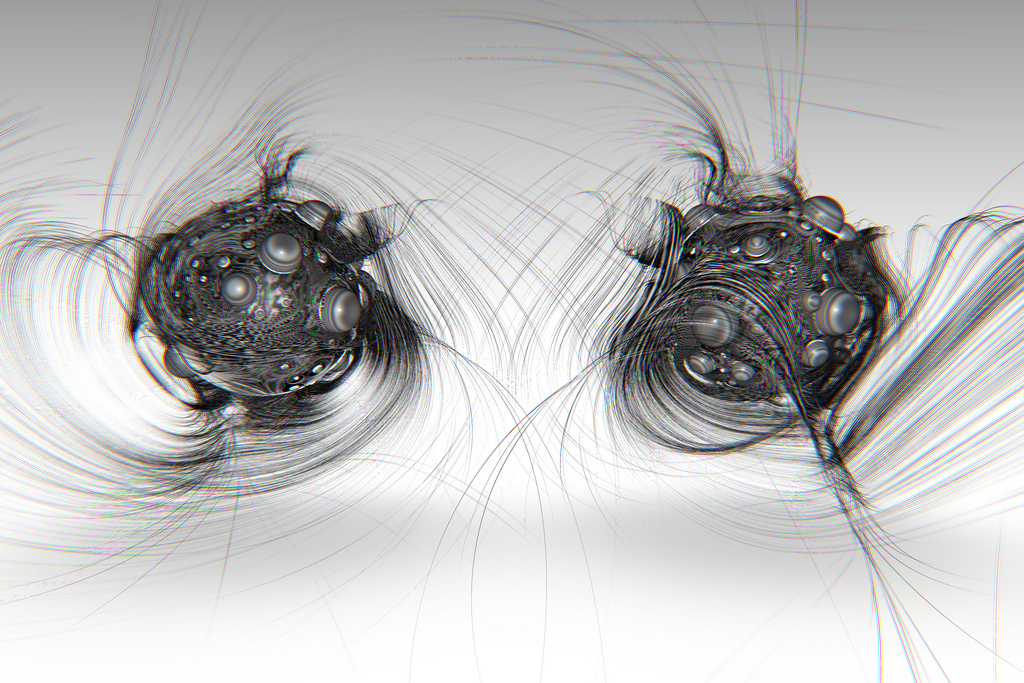
\includegraphics[width = 1\textwidth]{imgs/writtenimages.jpg}
\end{centering}

Ilustrace pochází z Hodginovi grafické práce, která byla vybrána jako jedna ze 42 prací do prvního vydání knihy {\em Written Images}.

Kniha je kurátorským projektem a samostatným výtvarným počinem dánského tvůrce \textbf{Marcina Ignace}. První výtisk knihy byl vydán v vydané v roce 2011. Samotná kniha je konceptuálním počinem, automatizací vychází každý výtisk s posunem o jedno okénko a tím ilustruje ducha generativní tvorby. Kniha je zpracována také softwarem Processing. \vfill

\begin{centering}
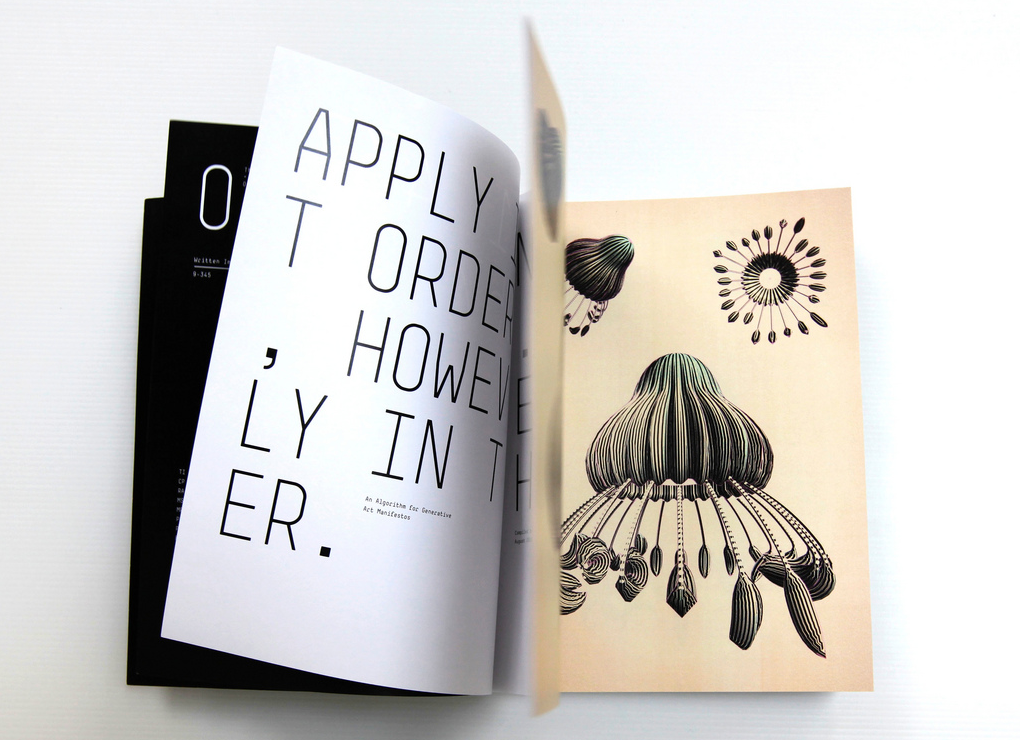
\includegraphics[width = 1\textwidth]{imgs/writtenimages.png}
\end{centering}

Kniha obsahuje generativní obrazy následujících umělců:
{\em 
386dx25, Antoni Kaniowski, Ariel Malka, Carl-Johan Rosén, Casey Reas, clone, David Bollinger, David Bouchard, e m o c, flight404, Golan Levin, Jonathan McCabe, Jörg Piringer, Julien Deswaef, Kim Asendorf, kraftner, Leonardo Solaas, Lia, Luke Sturgeon, Marcin Ignac, Marius Watz, Michael Zick Doherty, Mitchell Whitelaw, Moka, Nervous System, Oliver Smith, paolon, Perceptor, rhymeandreason, Ricard Marxer, Roberto Christen, Rui Madeira, Ryan Alexander, Ryland Wharton, Sansumbrella, sojamo, Stefano Maccarelli, Szymon Kaliski, Victor Martins, W:Blut, William Lindmeier, zenbullets} 










 

\newpage
\oddil{Idea Space - A Cyclic Universe}


\begin{center}
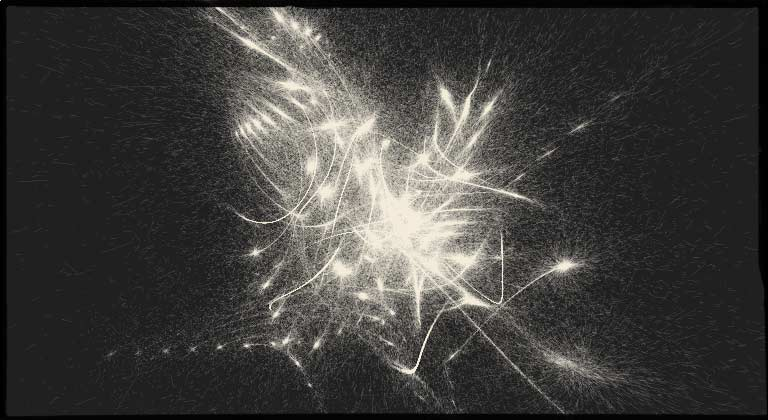
\includegraphics[width = 1\textwidth]{imgs/ideaspace1.jpg}
\end{center}

\begin{itemize}
\item
Autor: Karsten Schmidt
\item
Rok: 2004
\item
Médium: generovaná grafika - černobílý tisk
\item
Anotace:

Stills of an ongoing visualization project of a space with a steadily increasing number of moving particles attracted by slowly moving, invisible gravitational centres. the cyclic nature of the space itself acts as four dimensional history, causing each particle to leave a persistent trace in time as well as in space. the paradoxical result of this setup is that whereas the number of particles is approaching infinity there's no increase in computational cost.

As the particles move through space they become attracted by the various, initially randomly positioned gravitational centres. the force of attraction follows the classic "inverse square law" in physics, meaning a particle is a lot more influenced and accelerated by a close attractor than by ones further away. the more particles are in a highly active gravitational reqion of the space, the more clearly lines start to appear, showing the trajectory of these particles through space as well as time towards the locally strongest gravitational center.

\end{itemize}



%\end{comment}


\chapter{Cíle knihy}

\oddil{Konktrétní zadání}

Cílem této knihy je provést uživatele začátečníka sérií příkladů, které budou v průběhu ilustrovat znalosti nebytné k naprogramování postupných stádií programu. Jako první cíl si vytyčíme jednoduchý interaktivní program. Interaktivní program je takový, který dokáže určitým způsobem reagovat na uživatele. Tento program by ve výsledku měl přečíst polohu myši a na jeho základě provést proměnu v obraze.

Na úvod je třeba říci, že vytyčení konkrétního cíle není vždy nezbytné. Processing již počítá s možností, že uživatel nebude od počátku znát konkrétní zadání a bude jen volně experimentovat s funkcemi jazyka. Proto Processing automaticky pojmenovává nové projekty, v žargonu Processingu sketche, podle data svého vytvoření. (Více o sketchích \odkaz{Sketch}).


\chapter{Dobré zdroje v začátcích}

\oddil{Síť}

Autor knihy předpokládá že má čtenář v roce 2012 přístup ke globální síti internet.

Nejlepší reference pro práci s Processingem zůstává tato síť. Processing byl vyvinut síťovou komunitou a je také v síti nejlépe zdokumentován. Existuje několik dobrých obecných stránek s průvodci. Za všechny lze jmenovat domovskou stránku projektu {\em processing.org}. Zde naleznete téměř vše co by jste mohli potřebovat. Nacházejí se zde zdokumentované veškeré příkazy Processingu. Je zde i záložka {\em Learning} s jednotlivými průvodci do různých oblastí. 

Nejadresněji se vám dostane pomoci prostřednictvím webových fór nebo IRC kanálů. Na fórech se již řešil téměř jakýkoli problém, stačí proto vyhledávat klíčová slova vašeho konkrétního dotazu a velmi rychle by jste měli nalézt řešení.
 
   Na síti je dále obrovské množství uživatelů volně sdílících své programy včetně zdrojových kódů. Nejpočetnější komunita sídlí zřejmě na portálu openprocessing.org založeném a zpravovaném Sinanem Ascigolu.
   
Veškerá dokumentace je v angličtině včetně webových fór i dalších knih o programování. Nemáte-li problém s jazykem míst k zdokonalování se v Processingu bude vždy dostatek. \bublina{doporučuji se nejprve seznámit s projekty které jsou na internetu, získáte tím představu o tom, k čemu se vlastně Processing využívá}


\oddil{Examples - příklady přímo v Processingu}

Tato pomoc je vždy po ruce. Processing je navržený k výuce a je připraven poskytovat pomoc ze své podstaty. Přímo do aplikace Processingu jsou naimplementovány základní postupy v programování. Témata jsou pokrytá od základních operací až po pohyb v trojdimenzionálním prostoru nebo manipulaci s pixely.

Příkladů je zde dostatek a jsou přehledně uspořádány. Vřele doporučuji si je čas od času prolistovat.

Ke všem příkladům se dostanete z Processingu skrze nabídku {\em File > Examples} \odkaz{Základní prostředí}

\oddil{Knihy a průvodci}

Ano, jednoho průvodce právě držíte v ruce (nebo čtete na obrazovce). V minulosti vyšlo bezmála desítka podobných knih na toto téma. Jsou bezesporu obsáhlejší než kdy měla tato kniha v úmyslu.

Mezi všemi bych vám doporučil nejvíce původní knihu od samotných tvůrců Processingu Casey Rease a Bena Frye nazvanou {\em Processing: A Programming Handbook for Visual Designers and Artists}.

A rozhodně pak knihu Daniela Shiffmana {\em Learning Processing: A Beginner's Guide to Programming Images, Animation, and Interaction} je jednou z velmi podrobně napsaných knih o Processingu.

Knihy jsou vcelku dostupné a dají se opatřit přes internet. Rozhodně bych to doporučoval všem, kteří  potřebují mít opravdu dobrou dokumentaci vždy při ruce. V neposlední řadě bych také upozornil na to, že koupí knihy podporujete tvůrce svobodného softwaru, a tím potažmo i svobodný software jako takový. \odkaz{Otevřenost softwaru}

\oddil{Experiment}

Nejdůležitějším zdrojem vašich vlastních zkušeností bude vždy samotné experimentování s programováním. Na tuto část kladu největší důraz a v průběhu této knihy to i několikrát zopakuji, je vždy dobré odložit knihy a reference a pustit se do neznámých vod, zkušenost kterou takto naberete, bude vždy ta nejhodnotnější. Nebojte se proto sami experimentovat. \odkaz{Empirický přístup k programování} \bublina{příštích několik kapitol se věnuje obecnějším úvahám o programovacích jazycích, již nyní si můžete Processing nainstalovat}

\chapter{K čemu slouží programovací jazyk?}

\oddil{Počátky programovacího jazyka}

Výchozím bodem v tvorbě počítačové logiky jak ji známe dnes byla přirozená lidská komunikace v podobě řeči. Člověk používá jazyk  a při tvorbě zcela nového systému pravidel zákonitě sahá po známém prostředku.

Na počátku ale nebyl lidský jazyk. Se stroji se v jejich raných fázích vývoje hovořilo čistě strojovým jazykem, už v podobě číselných řad, nebo později holého strojového kódu, který přešel na logiku pokročilejších obvodů. Programovací jazyk se objevil již v padesátých letech minulého století a osvědčil se jako prostředek pro člověka, který začínal být limitován oproti kapacitě stroje schopného obsáhnout složitější úlohy. Řešením pro vzrůstající složitost logiky programů se stala lidská řeč.

Řeč se v počátcích tvorby struktur pro program jevila jako člověku nejpřirozenější řešení. Velmi brzy tvůrci zjistili, že za pomocí jazyka lze sice definovat složitý problém pro člověka, vyvstává tím ovšem problém definice významu takového jazyka stroji.

Počítačový jazyk není jeden, počítačových jazyků jsou celé rozvětvené rodiny. Konceptů, jak lépe hovořit srozumitelně pro člověka a zároveň ke stroji je celá řada, žádný z nich nedokáže kopírovat plně lidský jazyk v jeho přirozené struktuře. Důvodů je několik, jeden z nejpodstatnějších je fakt, že lidská řeč neodpovídá organizaci ve struktuře stroje, jednoduše proto že člověk své řeči sám nerozumí natolik, aby popsal sám všechny její zákonitosti logickou cestou.

Jednoduše řečeno lidský jazyk není popsán tak dokonale, aby jsme ho byli schopni vysvětlit stroji. Pokusy o průnik lidské řeči a logického obvodu sahají do absolutních počátků interakce člověka se strojem a představují pro tvůrce strojů závažný problém. Tento problém v padesátých letech minulého století definoval Alan Turning, jeden ze zakladatelů výpočetní techniky tak jak ji dnes známe. Alan Turning spolu s Gordonem Wechmanem stáli v době druhé světové války u vývoje dekryptovacího stroje německých šifer nazvaného Bomba {\em (The Bomb)}. Alan Turning v poválečné éře definoval formální rámec počítače jak jej známe dnes. Koncepce později nazvaná Turningův stroj vycházela zejména z matematických potřeb a jednalo se o snahu vytvořit kompletní výpočetní jednotku schopnou řešit veškeré známé matematické operace. 


Je pozoruhodné, že Alan Turning se již při raných stádiích vývoje počítačů zabývá takzvanou umělou inteligencí. Z toho je zřejmé, že stroje podobné počítačům se od počátku svého vývoje připodobňují struktuře lidského uvažování. Alan Turning sestavil pro stroje známý experiment nazvaný turningův test. Turningův test měl prověřit schopnosti stroje replikovat lidské chování, není náhodou že prostředek pro komunikaci v testu byla zvolena právě řeč. Test spočíval v modelové situaci stroje schopného napodobit lidskou komunikaci, tak dokonale aby člověk nebyl schopen rozeznat že komunikuje se strojem. Zajímavé na této definici lidské intelignece je zejména její vágnost, která v podstatě ilustruje míru porozumění logického uvažování lidské mysli jako takové.

K tomu, abychom sdělili informaci, používáme jazyk. Jazyk musíme umět přizpůsobit tomu, aby informoval, sdělil jistou skutečnost - myšlenku sdělovanému subjektu. Jazyk má nutně několik úrovní, zdaleka ne všechny jsme schopni reflektovat. Logicky popsaným jazykem a vnitřně uceleným systémem jsme schopni vysvětlit pouhý fragment skutečnosti.

Programovací jazyk je prostředek pro zápis algoritmů, jež mohou být provedeny na počítači. Zápis algoritmu ve zvoleném programovacím jazyce se nazývá program.





\oddil{Jednoduchý programovací jazyk}

Snaha po  zpřístupnění programování širší veřejnosti dala již na konci dvacátého století vzniknout rodině jazyků, které jsou patřičně zjednodušeny tak, aby je mohli obsluhovat i neodborníci.

Zjednodušení programování je odpověď na situaci, kdy programovací jazyky vytvářeli především lidé se zvláštním nadáním pro ryze technické uvažování. Pro technické uvažování nemá každý člověk správné predispozice. Programování dnes znamená především určitý stupeň svobody při komunikaci se strojem.

K míře svobody, která má své silné kritiky\footnote{včetně mne samotného}, se nyní nechci vyjadřovat, ale zjednodušeně z pohledu pouhého uživatele který používá daný nástroj, schopnost programovat činí z uživatele již potencionálního strůjce vlastních nástrojů.

Hovořím-li o stroji, mám dnes na mysli spotřební počítač. Termín \slovnik{stroj} používám záměrně pro zdůraznění jisté formy strojového přemýšlení v historickém kontextu.

Nástroje jsou pak programy zkonstruované pro jistou činnost. Nástroj je obvykle vyvíjen za jedním účelem, který plní uživatelsky co nejpřívětivější cestou. Tato cesta je pro uživatele snadno schůdná a nabízí mu standartní škálu dovedností nástroje.

Aniž bychom si to často uvědomovali, současná vizuální kultura je ovlivněna těmito nástroji daleko více, než je na první pohled zřejmé. Technické možnosti jsou současným tržním hladem pro inovaci patentovým systémem vlastněny a proměňovány ve zboží. V této situaci je důležité znát nástroje i jejich vznik pro reflexi nebo kritiku v širších souvislostech.

Tato kniha je spíše než-li jednomu nástroji věnována programu pro tvorbu takových nástrojů. Jak již vyplývá z této definice, použití Processingu není limitováno jen úhlem pohledu autora tohoto textu. Návod by se měl stát spíše pobídkou k co nejrozmanitější tvorbě vlastních nástrojů, sloužících opět k co možná nejširší škále možných účelů.

Processing vychází z koncepce snadného přístupu k programování. Za běžných okolností by se vnímavý člověk měl být schopen naučit jednoduché struktuře programu a schopnosti vytvořit vlastní program v průběhu několika dní. Na druhou stranu, právě predispozice našeho uvažování jsou natolik rozmanité, že takovou prognózu nelze brát jinak než jen za orientační.




\oddil{Dokonalost jazyka}

Co je to dokonalý jazyk? Nejprve je zapotřebí říci, že absolutně dokonalý jazyk neexistuje. Jazyk si můžeme představit jako systém vzájemných vztahů, který je schopen popsat jednotlivé symboly nebo objekty. Symboly můžeme nazvat předměty, tyto předměty dále mají své vlastní hodnoty a vlastnosti, jazyk kromě definic takových vlastností operuje a popisuje jednotlivé jevy a vztahy mezi těmito předměty. Jednodušší popis jazyka je v pojetí výpočetní techniky určitý ucelený systém schopný popsat rozmanité problémy řešitelné strojem.

Co předem činí jakýkoli jazyk absolutně nedokonalým je nejprve fakt, že jakýmkoli jazykem nedokážeme vyjádřit původ jazyka, tj. jeho strůjce; člověka. Jazyk použitý pro instruktáž stroje je vnitřně konzistentní a funguje logicky hermeticky, tj. nepřipouští jiný než jeden výklad konkrétního textu. Pojetí dokonalosti jazyka ve smyslu vnitřní logické konzistence je naprostou nezbytností v pojetí interpretace strojem, na druhou stranu téměř nepřekonatelnou překážkou v případě abstraktnějších úvah o programování jako takovém.

Použiji zde pro názornost rozdíl programovacího jazyka s jazykem českým. Český jazyk, stejně tak jako jakýkoli mluvený nebo psaný jazyk, je jazykem organický ustáleným po staletí užívání. Jazyk jak ho známe slouží ke komunikaci mezi lidmi, lze tedy použít například pro popis krajiny. Přestože k dokonalému popisu krajiny stěží kdy můžeme dojít, slovy které se opírají o určitou sdílenou zkušenost, lze poměrně dobře přiblížit určitý obraz věcí.

Kdy bychom se pokusili pro popis krajiny použít jazyk programovací, dostaneme se velmi rychle do nesnází. Programovací jazyk není jazykem určeným pro předání informací mezi lidmi, ale pro komunikaci člověka se strojem. Jeho vnitřní logická konzistence, tvrdá logická struktura, která nedovoluje v jeden okamžik jinou než jednu interpretaci, je jeho velikou předností při definici exaktních parametrů. Podobnost s řečí spočívá ve vazbě slov, které reprezentují jednotlivé hodnoty a operace. Hlavní odlišnost je v jeho syntetickém původu, jedná se o jazyk umělý. Programovací jazyk je přednostně zkonstruovaný pro definici známého a pochopeného. V případě neznámých nebo nepoznaných veličin, je programovací jazyk víceméně k ničemu. 

Chceme-li komunikovat se strojem, musíme tedy svůj způsob vyjadřování přizpůsobit logicky dokonalému jazyku - vnitřní logice fungování stroje. Počítač není navržen k tomu, aby něčemu rozuměl. Počítač je navržen k řešení jasně definovaných otázek. Tato kniha se pokusí srozumitelnou formou popsat jeden z možných způsobů jak si takový jazyk osvojit a potažmo způsob uvažování, který vede k jasné definici problému. Hovoříme-li o programování, máme na mysli proces tvorby jisté logické struktury. Osvojení si programování spočívá ve schopnosti definovat problém nebo jasně formulovat otázku tak, aby stroj na ni mohl odpovědět.

Vtip celé věci spočívá v tom, že ovládneme-li formálně jazyk určený stroji, můžeme prostřednictvím tohoto stroje hovořit i ke člověku, tj. popisovat i pocity z rozkvetlých luk.

\oddil{Volba vhodného jazyka}

Ve výpočetní technice se nachází celá škála programovacích jazyků i prostředí. Tyto jazyky mají svoji genezi a byli historicky vyvíjeny především počítačovými odborníky. Jejich dokonalost lze těžko ocenit z vnějšího pohledu, a to právě z důvodu jejich konstrukce, která odpovídá a částečně podléhá určitým účelům, ke kterým byli tyto jazyky původně navrženy. Celistvý pohled na vývoj programovacích jazyků zde není možné obsáhnout. Základní rozdělení programovacích jazyků dle historického vývoje můžeme označit na dvě skupiny, jazyky imperativní a objektově orientované.

Processing se svojí stavbou na základech Javy řadí k objektově orientovaným jazykům. Jeho společnými příbuznými jsou tímto rozdělení kromě {\em Javy} jazyky jako {\em Perl, Smalltalk, C++, Object Pascal, C\#, Visual Basic .NET, PHP, Python, Ruby} nebo {\em Lisp}} Toto rozdělení pojednává o metodice jazyka jako systému vzájemně působících objektů. 

Rozdíl mezi imperativním pojetím programování a objektově orientovaným pojetím spočívá především v logice kódu a jeho následném uspořádáním. Imperativní jazyk se dá považovat za předchůdce objektově orientovaného pojetí. Nedá se obecně tvrdit, který přístup je výhodnější, jedná se o dvě rozdílná paradigmata. Dnes mezi nejpoužívanějšími programovacími jazyky masivně převládá objektově orientované paradigma.

Rozdílné pohledy lze ilustrovat na popisu nějakého jevu. Jev se dá popsat různými způsoby. Jedna perspektiva bude více hovořit o aktérech jevu, ty rozdělí do objektů a jejich vlastností a možností. Druhá perspektiva popíše celistvou situaci jako sérii událostí, které je možné v tomto pořadí kdykoli zopakovat.


V posledních přibližně dvaceti letech se mezi programovacími jazyky postupně objevuje tendence po větší srozumitelnosti a potažmo zjednodušení programování jako takového. Programování v této koncepci již není jazykem odborníků, ale je demokraticky přístupné širší veřejnosti z rozmanitých - prioritně netechnických oborů.

Tato tendence postupně dala vzniknout celé rodině programovacích jazyků, které se snaží přiblížit potenciál výpočetní techniky netechnickým oborům, v neposlední řadě i oborům výtvarným. V technických kruzích je ovšem již sama disciplína psaní programů považována za tvůrčí činnost. V pojetí výtvarného umění dnes převažuje pohled na programování jako na velmi technickou zdatnost, rigidní a notně limitovanou činnost.

Jazyk, který je nutně limitovaný svojí nezbytnou dokonalostí, ovšem nemusí nutně limitovat svého uživatele ve sdělení. Uživatel se ovšem musí  k uskutečnění takové zdárné komunikace přizpůsobit stroji.


\oddil{Proč zrovna Processing?}

Processing je vhodný nástroj pro první experimenty s programováním z několika důvodů.

Prvním důvodem je jednoduchost směrem k uživateli, Processing se snaží začátečníky co nejméně zatížit zbytečnými informacemi. Processing prezentuje programování jako přístupnou a ovládnutelnou schopnost. Processing toho dosahuje především rychlou odezvou vizuálního prostředí. Jednoduše řečeno v momentu kdy spustíme kód vidíme okamžitě jeho vizuální výsledek. Taková ilustrativnost je v začátcích podle mého názrou téměř nezbytná.

V Processingu lze velmi krátkým kódem programovat sofistikované programy. Pro příklad zde uvedu soutěž nazvanou {\em Tiny Sketch} pořádanou portály Rhizome.org a Openprocessing.org. \bublina{máte-li počítač u sebe a jste-li připojeni k internetu, vřele doporučuji si nyní projít aktuální podobu stránky openprocessing.org} Processing dokáže být natolik úsporný, že za pomoci maximálně dvouseti znaků, zde byli tvůrci schopni naprogramovat svébytné programy.

\vfill

\begin{center}
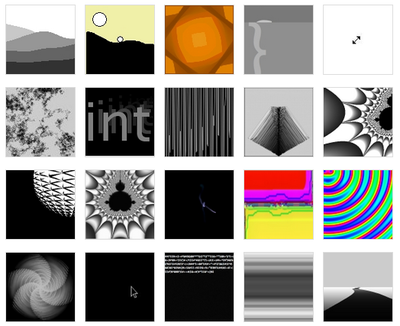
\includegraphics[width = 1\textwidth]{imgs/tinysketch.png}
\end{center}



Snad největší předností pro začínající programátory je výtečná dokumentace a velmi přívětivá komunita lidí poskytující neúnavně rady začátečníkům.


\oddil{Tvorba softwaru}

Programy jsme dnes zvyklí spíše využívat než sami vytvářet. Vytváření programu je náročný proces a tvorba uživatelsky přátelského prostředí pro tvorbu programu je složité.

Processing se svým způsobem neliší od žádného jiného programu, který běžně využíváme. Jedná se o sadu příkazů a samotné programovací prostředí, které nám dovoluje určitou formou vytvářet svébytný program. I když se jedná již o programování, nelze jej běžně zaměňovat s klasickou tvorbou dospělého nástroje.

Zde si musíme uvědomit, že náš potencionální produkt - program bude vždy spíše banální v porovnání se samotným prostředím Processingu. Procesingový kód je výčet všech možností, které můžeme při tvorbě našeho programu využít. Obecně se dá říci, že Processing je nástroj pro tvorbu speciálních nástrojů. Výsledek našeho programování bude vždy pravděpodobně obsahovat poměrně větší část Processingu samotného.

Je dobré od začátku pochopit, k čemu lze Processing využít a k čemu jej opravdu využívat chceme. Processing se především hodí k rychlé tvorbě programu, ověření teze nebo spontánního nápadu. Pro podobné programování se také vžil pojem "rapid engineering". Tvorba dospělejších nástrojů není sice nemožná, obecně ale platí, že Processing bude svými zkrácenými zápisy a jednoduchostí prostředí velmi nápomocný v začátcích. 

Processing se svojí konstrukcí zejména hodí pro práci s obrazem a tedy obrazu bude také věnována nejrozsáhlejší část této knihy. Výstupy z Processingu lze nadále zpracovávat, Processing může tak sloužit například jako mezičlánek ve výrobním procesu.

Dnes je Processing zejména využíván grafickými designéry, designéry užitého umění, tvůrci webových aplikací, softwarovými návrháři, vizuálními umělci a umělci kteří se věnují instalacím v prostoru nebo živé projekci. K Processingu si ovšem nacházejí cestu i více technické obory, zejména architekti, badatelé přírodních věd, statistici a všeobecně tvůrci softwaru, ale Processing nachází využití i v oborech zabývající se humanitními vědami jako například sociologové nebo jazykovědci.

Processing se neomezuje na jeden obor, svojí koncepcí spíše nabízí společnou platformu pro mezioborovou komunikaci.


\pododdil{Otevřenost softwaru}

Processing je jedním z jazyků, který byl vytvořen v diskurzu zjednodušování programování. Jako každý jiný programovací jazyk je i Processing navržen pro jisté účely. V případě tohoto programovacího jazyka se nejvíce jedná o důraz na rychlý vývoj a zjednodušené nakládání s obrazem i prostorem. Z více technického pohledu pak Processing vyniká otevřeností zdrojového kódu a důrazem na multiplatformnost.

Z pohledu vývojáře je velmi důležité, že jazyk i programovací prostředí Processing je v současnosti \slovnik{otevřený software}, což znamená, že prostředí i samotný zdrojový kód je volně k dispozici. Processing je dále šiřitelný pod \slovnikpl{MIT licence}. Pro vývojáře otevřenost zdrojového kódu znamená zásadní věc, jednoduše pro dosažitelnost celého zdroje, který se dá následně například implementovat do různých prostředí. Další možnost vývojáře je rozšířit jazyk o vlastní funkce, a tím participovat na projektu, například tvorbou takzvaných knihoven. \odkaz{Knihovny} Otevřenost kódu teoreticky navyšuje počet možných participantů a de facto celý projekt udržuje v dlouhodobém horizontu naživu.

Z pohledu samotného uživatele je velmi příjemné, že samotný software je k dostání zdarma na stránkách projektu. Za jeho užívání není nutné platit žádné poplatky, a to i v případě komerčních užití. V případě potřeby vyjádření vděku za práci autorů je možné zmínit kdekoli ve Vašem produktu \slovnik{Built with Processing}. \bublina{v začátcích nemusíte věnovat velikou pozornost této zvyklosti, dostane-li se vám po čase dobré pomoci z komunity, nebo budete-li jednoduše Processing využívat ke své práci, můžete jej někde zmínit, a tím vlastně projekt podpořit}


Processing na první pohled není ničím zvláštní programovací jazyk. V podstatě by se dalo říci, že se jedná pouze o rozsáhlou knihovnu původního jazyk Java.


To, co Processing řadí mezi oblíbené softwary pro tvorbu, je nejvíce přívětivá komunita uživatelů s velmi odlišnými stupni znalostí a úhly pohledu. Zvláštní důraz je v komunitě kladen na poskytnutí co největší podpory právě začínajícím uživatelům. Tomu odpovídá i počet rozmanitých průvodců a rozsáhlá, velmi dobře a stručně napsaná dokumentace ke každému z příkazů v Processingu.

K otevřenosti v kódu v neposlední řadě přistupuje i celá řada velmi zkušených tvůrců. Tím se uživatel na jakémkoli stupni znalostí může kdykoli naučit nové postupy nebo může svobodně recyklovat algoritmy druhých uživatelů. Processing a čím dál více jeho uživatelů ctí filosofii otevřeného softwaru, která (mimo jiné) hlásá: \uv{Vědomosti nesmí být privatizovány!}

\pododdil{Syntetický obraz}

Hlavní doménou Processingu je schopnost vytvářet \uv{živé} programy, tj. programy běžící v reálném čase. Již jméno programovacího jazyka Processing napovídá akcent v čase se odvíjejících události.

Obraz vytvořený tímto způsobem, na první pohled zaměnitelný s videem, nemusí například podléhat časové omezenosti, nebo může určitým způsobem reagovat na své okolí. Obecně jev běžícího programu v čase můžeme pojmenovat Generovaný obraz (nebo zvuk). Rozdělení je zde trochu problematické, v případě digitálního obrazu se již dnes nejedná o nic jiného než generovaný obraz. Sám proto radši používám výraz {\em syntetický obraz}. Syntetický obraz je takový obraz, který byl vytvořen uměle, tedy skladbou logických prvků, za účelem je vizuálně reprezentovat. 


\pododdil{Empirický přístup k programování}

	I když bychom zásadní odlišnost s jinými programovacími jazyky hledali stěží, Processing proslul zejména snadností použití. Kompilovat program není otázkou nastavování kompileru a veškerých jeho parametrů, program jednoduše po stisku tlačítka {\em RUN} běží (je-li správně napsán). Samozřejmě tento redukcionistický přístup má své nevýhody, speciálně při rozsáhlejších projektech tato jednoduchost může dokonce omezovat. Processing ovšem jako svobodný software lze naimplementovat do řady jiných prostředí, a potřebujete-li si kompilační proces nastavit sami, nic vám například nebrání použít Processing jen jako knihovnu do {\em Javy}.

Tato jednoduchost na druhou stranu nezdržuje uživatele od myšlenkového toku psaní programu. Častou kontrolou výsledku kódu uživatel může lépe sledovat postupné změny v programu.

Nazývám tento způsob programování empirický, tedy přístup, kdy podle zkušenosti s běžícím programem je dotvářen i samotný zdrojový kód. Mnoho technicky zaměřených lidí by zřejmě mohlo tento postup kritizovat pro přílišnou reduktivnost a amatérský přístup. Zde bych oponoval faktem, že motivace lidí vytvářejících například instalaci do galerie, nezajímá příliš dokonalost (když už tedy vůbec) programu. Program je v pojetí tvůrců jen prostředníkem pro další sdělení, a jestliže toto sdělení předá, je to dobrý program.

Proces poznávání struktur jazyka při tvorbě obrazu prostřednictvím Processingu bych přirovnal k postupu od začátečnické malby na tkaninu k postupnému tkaní gobelínu. Zde je nutno podotknout, že ne každý tvůrce využívající Processing \bublina{Zamyslete se, k čemu by jste Processing rádi využívali, účel světí prostředky, v Processingu tomu bývá bohužel často právě naopak.} chce tkát gobelín a najde-li nástroj vhodný \uv{jen} pro \uv{malbu} na plátno, je to dobrý nástroj.


\chapter{Processing jako prostředí}


Processing představuje ucelené programovací prostředí tzv. PDE\footnote{Processing Development Enviroment}. Jedná se o kompletní prostředí určené především k rychlému vývoji aplikací. Samotný program je jednak otevřeným softwarem\footnote{tj. s otevřeným veřejně dostupným zdrojovým kódem}, a také zdarma ke stažení pro všechny majoritní platformy. Processing je k dispozici pro \slovnik{GNU / Linux}, Mac OS i pro Microsoft Windows na stránkách projektu processing.org. Porcessing je teoreticky možné spustit v jakémkoli prostředí umožňujícím chod virtuálního stroje Javy. Celý jazyk i samotné PDE vychází pod licencí \slovnik{GNU / GPL}, jedná se tedy o svobodný software \odkaz{Otevřenost softwaru} . 

\oddil{Základní prostředí}



\begin{center}
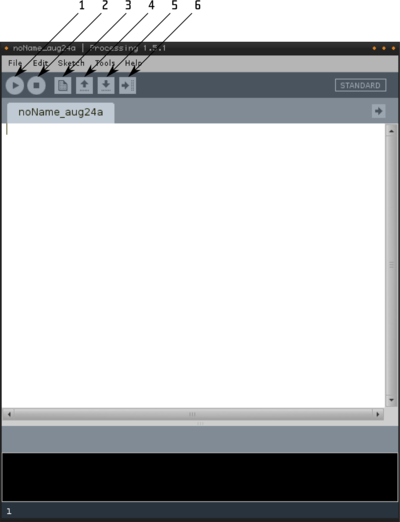
\includegraphics[width = 0.8\textwidth]{imgs/processing.png}
\end{center}


Základní rozhraní tvoří textový editor s několika nezbytnými funkcemi. Patrně nejdůležitější je v liště tlačítko (1) tzv. RUN. Které kompiluje a spouští program aktuálně rozpracovaný v textovém editoru. (2) Tlačítko STOP naopak program zastaví. V případě chyby v programu lze též využít jako vynucené zavření programu. Zbylé tlačítka slouží k diskovým operacím.\bublina{Zkuste nyní spustit Processing, bude dobré ho mít nyní při ruce, nemáte-li jej po ruce, doporučuji přeskočit následující kapitoly věnované prostředí}


\begin{center}
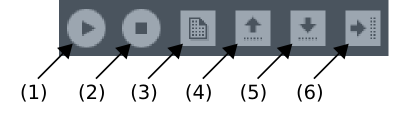
\includegraphics[width = 0.6\textwidth]{imgs/buttons.png}
\end{center}

\pododdil{Základní diskové operace}

Ty operace jež něco zapisují či načítají z disku. Tyto operace zahrnují veškerou manipulaci se sketchí, její vytvoření, uložení, načtení či export do webového formátu či kompilaci do spustitelné aplikace.

Processingová sketch nemusí být nutně uložena aby jste ji mohli spustit. Nové úpravy, které v textovém poli napíšete budou dočasně uloženy v závislosti na vašem operačním systému jinde. Tímto způsobem můžete experimentovat s kódem aniž by jste přišli o předchozí verzi.

Mezi základní operace patří vytvoření nové sketche (3), otevření předešlé (4), uložení (5) a export (6).

Tlačítka mají dále speciální vlastnosti s podržením tlačítka tlačítko s novou sketchí otevře také nové okno editoru. V kombinaci s načtením předchozí sketche (4) otevřete též sketch v novém editoru aniž by jste ztratili předchozí okno. U uložení se modifikace projevuje funkcí uložit jako. U exportu stisknutím klávesy \klavesy{SHIFT} přepínáte mezi exportem samostatné aplikace nebo tzv. appletu, aplikace schopné běžet v prohlížeči nebo obecně na webových stránkách.


\pododdil{Sketch}

Sketch je v Processingu označení pro jednotlivé projekty. Sketch je ve své podstatě složka obsahující alespoň stejně jeden stejně nazvaný soubor s příponou {\em *.pde}. Sktech při vytvoření nevyžaduje název, je jí přidělen pouze aktuální datový kód zaznamenávající datum vytvoření. Tímto decentním způsobem Processing toleruje například nejasnost záměru autora při vytváření nového díla, jeho název či pracovní název lze tímto způsobem přiřadit až později, po nabytí jasnějších obrysů.

Program si vystačí pouze se samotným zdrojovým kódem tj. souborem (soubory) {\em *.pde}. Ovšem v případě operujeme-li s externími daty stojícími mimo zdrojový kód, jakékoli jiné soubory, můžeme využít dvě možnosti. První možnost je soubor, se kterým potřebujeme operovat tažením myši přesunout na textové pole Processing \index{IDE}IDE. Touto operací bude soubor zapsán do naší sketche automaticky. Druhá možnost je operaci provést manuálně, stačí vytvořit v adresáři sketche adresář s názvem \slovnik{DATA}. Processing tuto složku automaticky rozpozná a soubory v této složce budou dobře dostupné pro pozdější operace.

Ke standartním adresářům, které se často objevují ve struktuře skteche, si stačí zapamatovat jen dva již zmíněný adresář nazvaný {\em DATA}. Tento adresář je využíván při práci s jakýmikoliv vnějšími daty jako jsou např. obrázky, zvuky, videa, vektorové grafiky nebo například textové soubory. Druhý adresář nazvaný {\em CODE} obsahuje externí zdrojový kód, popřípadě kód kompilovaný v podobě knihovny, mající nejčastěji přípony {\em *.java, *.class, *.jre}. Tento adresář se nalézá v systémové cestě daného projektu a umístíme-li zde soubory budou též dobře dostupné z daného projektu. Adresář {\em CODE} nás zatím nemusí příliš zajímat, později se jeho prostřednictvím můžeme pokusit rozšiřovat funkce Processingu externím kódem.


\pododdil{Sktechbook}

Místo na disku, které Processing využívá k uskladnění sktechí se nazývá povšechně sketchbook a je v podstatě pouze adresář obsahující jednotlivé projekty. Koncepce sketchbooku spočívá v uspořádání jednotlivých projektů do organizované formy a ačkoli nevnáší do jednotlivých projektů sám o sobě řád může napomoci k vytvoření řádu vlastního. Ze své zkušenosti mohu říci, že organizace jednotlivých projektů do jakékoli struktury má opravdu smysl. Mnou preferovaná struktura obsahuje jednotlivé roky následně ještě dělené do měsíců, ale možnosti organizace záleží čistě na uživatelových preferencích. Tímto chci spíše ilustrovat možnosti uspořádání než-li nezbytnost, ale přítomnost vašeho systému od počátku vřele doporučuji.

Ve sketchbooku se dále nachází jeden speciální adresář nazvaný {\em libraries}. Adresář v sobě uchovává externí rozšíření Processingu o komunitní knihovny. Standartně Processing již své základní knihovny nese v sobě, tj. jsou standartně přidány do samotného Processingu. V tomto adresáři se nacházejí knihovny které budete moci použít později. Na stránkách projektu {\em http://processing.org} můžete nalézt velké množství komunitních knihoven s dobrou dokumentací, volně ke stažení. Veškeré tyto knihovny tedy Processing potřebuje nalézt v tomto adresáři.






\pododdil{Editor}

Editor je textové pole a je vaším hlavním komunikačním nástrojem s Processingem. Veškeré informace které zadáte do tohoto pole budou interpretovány samotným Processingem. Textový editor není nijak dokonalý, pro začátek si s ním ovšem vystačíme. Formát který tento editor produkuje je ve své podstatě textový soubor s příponou {\em *.pde}.




Textový editor má několik funkcí, které vám mohou usnadnit práci. Odlišuje například mezi příkazy Processingu odlišnými barvami, tato zdánlivá drobnost speciálně v začátcích napomůže nebo v případě objemnějších kódů může výrazně zpřehlednit organizaci programu. Jedná se o programátorskou konvenci obecně v anglickém jazyce nazývanou \slovnik{syntax highlighting}.


Další konvencí se kterou se často setkáte je tzv. \slovnik{indenting}, zarovnávání kódu do úhledných paragrafů. V Processingu si ze začátku vystačíte se standartím zarovnáním, posléze lze zarovnávání aktivovat stiskem kombinace kláves \klavesy{CONTROL (APPLE) + T}.


\begin{center}
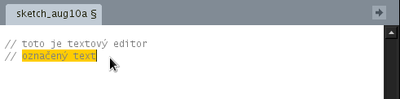
\includegraphics[width = 1\textwidth]{imgs/editor.png}
\end{center}

Horní lišta editoru označuje záložky, kliknutím na šipku v na pravé straně lišty se vám zobrazí možnosti operací se záložkami. Pro začátek s nimi nebudeme operovat. V případě delšího kódu záložky slouží k lepší organizaci struktury programu. V podstatě se dá říci, že každá záložka odpovídá jednomu souboru ve sketchi. Co je to sketch popíšu níže.

Jak můžete vidět na obrázku editor operuje i českými znaky, ačkoli bych jejich používání z důvodů internacionalizace neradil používat. V komentářích tj. textem uvozeným dvěma dopřednými lomítky {\em //}, tedy text, který kompiler ignoruje, jsou diakritická znaménka přípustná.

Naopak v případě názvu proměnných, nebo jakýchkoli funkčních definic, je použití diakritiky v devadesáti procentech nefunkční.\footnote{standartní jazykové kódování, ve kterém Processing operuje je {\em UTF-8}}


\oddil{Klávesové zkratky}

\begin{itemize}
\item[\klavesy{CTRL + r}]  spustí program
\item[\klavesy{CTRL + SHIFT + r}] takzvaný present mode spustí program a zatemní zbytek obrazovky
\item[\klavesy{CTRL + t}] automatické formatování textu, zarovnavá text do odrážek
\item[\klavesy{CTRL + k}] otevře adresář konktrétního projektu
\item[\klavesy{CTRL + f}] vyhledávání v textu a nástroj pro hromadné nahrazování
\item[\klavesy{CTRL + SHIFT + f}] vyhledávání v označeného příkazu v referencích
\item[\klavesy{CTRL + s}] save, uloží projekt na disk
\item[\klavesy{CTRL + SHIFT + s}] uložit jako

\item[\klavesy{CTRL + e}] export jako webový applet, otevře exportovaný projekt
\item[\klavesy{CTRL + SHIFT + e}] export jako aplikace, zobrazí okno s výběrem platform pro export

\end{itemize}

* značí klávesu \klavesy{CTRL} PC a \klavesy{APPLE} na Mac.


\chapter{Processing jako jazyk}

\oddil{Soustředěná činnost}

Než začneme doopravdy programovat musíme si uvědomit, že tento proces vyžaduje velikou dávku koncentrace. Obecně se nedá říci jaké fyzické prostředí je k programování ideální. To se samozřejmě může lišit. Obecně platí, že fyzický prostor, který k programování potřebujete je prostor, ve kterém se můžete sami soustředit na práci.

Koncentrace při psaní programu je specifická dovednost, kterou se začátečník učí jen stěží. Bohužel pouhým čtením této knihy se již vyvádíte z potencionální koncentrace. Učení se programovat je náročný proces a vyžaduje velikou dávku koncentrace sám o sobě. Okamžité vyzkoušení nových poznatků pomáhá zápisu informací do vaší dlouhodobé paměti a opakování je samozřejmě nezbytné k utužení těchto struktur. Co je bohužel při počátečním programování nezbytné je například hledání v referencích a spolu se soustředěním na program samotný je celý proces učení se na koncentraci velmi náročná věc.



V problematice programování obecně platí, že není nic složitějšího, než číst cizí kód, nebo dokonce kód vlastní s odstupem času. Při programování se lidská mysl dostává do stavu mimořádné bdělosti a koncentrace. Tento stav je často popisován programátory jako tzv. \slovnik{flow}. Jendá se o stav, ve kterém mysl vědomě udržuje celý program\footnote{nebo větší části programu} v paměti.

Pokaždé když si programátor takový stav přivodí, vše v kódu\footnote{podle míry ovládnutí programovacího jazyka} se pro něj jeví srozumitelné. Formátování a standarty velmi napomáhají k rychlému navození bdělého stavu, protože sami o sobě jsou jistou formou jazyka.

\oddil{Základní pravidla a zvyklosti}

V programování obecně platí jisté zákonitosti. Není tomu jinak i u pravidel, které nejsou důležité pro čtení kódu strojem ale pro člověka. Speciální zákonitosti formátování kódu mají ryze praktickou funkci. Jedná se o standart dodržovaný programátory, tak aby mezi sebou byli schopni sdílet své úsilí. \bublina{otevřte nějaký z příkladů z lišty file > examples, a letmo se seznamte s kódem jak vypadá, i když mu nebudete rozumět podívejte se jaké znaménka a barvy se v kódu opakují atd.}
  
  
\oddil{Logika programování}
Pro začátek je dobré si představit program jako sadu instrukcí. Každá instrukce má svůj význam a své místo. Instrukce se píší v programovacím jazyku a jejich interpretace je vždy pro stroj jednoznačná. Stroje podle svého návrhu nedělají nic kromě toho co mají takovým způsobem instruováno.

Veškeré programy které používáte, dokonce i programy, které nevíte že používáte byly někdy naprogramovány lidmi pomocí programovacích jazyků. Programovací jazyk je pouze, plánovací forma zápisu programu. K tomu, aby byl program spuštěn, musí být v případě jazyku Processing převeden do strojového kódu. Strojový kód se liší od toho zdrojového, našeho čitelného plánovacího jazyka, tím že není čitelný pro člověka, je čitelný pro stroj.

Počítač je pouhý stroj. Umí dnes opravdu rychle vykonávat sled banálních operací. Programovací jazyk slouží k vytvoření smyslu ve sledu banálních operací. Procesu převodu ze zdrojového kódu do strojového se nazývá kompilace.

O kompilaci toho nemusíme naštěstí vědět mnoho, vše bylo již tvůrci Processingu a jazyku Java shrnuto pod tlačítko spustit.\bublina{budete-li mít otevřený nějaký kód z examples, zkuste ho nyní spustit, uvidíte jak se program chová, vyzkoušejte několik příkladů}

\newpage
\chapter{Stavba programu a syntax}



\pododdil{Kometář}
\label{komentar}

Komentář je vše co program ignoruje. Je to místo v programu učené ke čtení člověku. Kometáře dále často slouží k rychlé editaci programu. Odkomentováním řádky funkčního kódu lze vynechat některé funkce Processingu.


Nádsleduje zápis tak, jak jej již můžete vepsat do editoru Processingu. Vřele doporučuji mít v této chvíli Processing v průběhu čtení knihy zapnutý a po ruce, aby jste si příklady v rámečcích mohli vyzkoušet. Komentář je řádek textu, nebo její část uvozená dvěma dopřednými lomítky.


\begin{lstlisting}
// komentar je uvozen dvemi doprednymi lomitky
\end{lstlisting}

Spustíte-li nyní program tlačítkem RUN, objeví se šedé okénko prvního Processingového programu. Jelikož jste zatím nedefinovali nic funkčního, program také nic nedělá.

V praxi je pak často využívaný i druhý způsob komentáře, takzvaný víceřádkový komentář. Ten začíná dopředným lomítkem a hvězdičkou a končí těmito znaky v obráceném pořadí.

\begin{lstlisting}
/* viceradkovy komentar je uvozen
doprednym lomitkem a hvezdickou
ukoncen hvezickou a lomitkem 
(v obracenem poradi)

toto je viceradkovy KOMENTAR
toto je viceradkovy KOMENTAR
toto je viceradkovy KOMENTAR
toto je viceradkovy KOMENTAR
*/

/*zacatek .............. konec*/

\end{lstlisting}

Komentáře v Processingu poznáte vždy nejrychleji tak, že je bude editor obarvovat šedou barvou. \bublina{vyzkoušejte si napsat nějaký text do textového editoru, spusťe program, následně před něj vložte dvě dopředná lomítka, pozorujte rozdíl}

\pododdil{Základní datatypy}

Ke stavbě programu potřebujeme stavební materiál. Pro základní pochopení fungování programu je nezbytné nejdříve pochopit základní datatypy. Datatyp si lze obecně představit jako obálku na informaci.

Processing rozlišuje mezi jednotlivými datatypy. Informace, které se nacházejí v paměti se musí nacházet pod správným datatypem, tak aby program věděl jak s nimi operovat.

Pro datatyp je možné představit si různé paralely, má oblíbená je podobnost s obálkami nebo nádobami. Různé datatypy si můžeme představit jako tvary nádob. Do různých nádob, lišících se tvarem, se směstná různý obsah. Typy obsahů se dají názorně představit na rozdílu mezi textovou informací a informací číselnou.

Processing potřebuje nejdříve vědět zda nádoba obsahuje text nebo číslo, aby mohl s touto nádobou operovat. Například, nelze provést matematickou operaci mezi dvěma slovy. Sčítat, odčítat, dělit či násobit se dají pouze čísla.


\pododdil{Seznam základních datatypů}
Datatypů je jen několik, dají se vcelku snadno zapamatovat:

\begin{lstlisting}
int mojeCeleCislo = 1;

float mojeCisloSDesetinnouCarkou = 1.33;

boolean mojePravdaCiNepravda = true;

String mujSlovniRetezec = "Ahoj svete!";

char mujJednotlivyZnak = 'A';

\end{lstlisting}

Takovému zápisu bude již Processing rozumět. Vepsáním těchto řádků do processingového editoru již dochází k alokaci vašich informací ve správných datatypech v paměti. Vysvětleme si nyní několik nejasností.

První slovo na každém řádku označuje odlišný datatyp (náš tvar nádoby), následuje jméno proměnné (název pro naší nádobu), poté následuje rovnítko které již přiřazuje obsah - hodnotu do proměnné (nádoba je naplněna).

Každý příkaz je ukončen středníkem {\em ;} .

Podivné názvy jako například {\em mojeCeleCislo} tzv. proměnných, jen ukazují, že název pro svoji proměnnou můžete zvolit téměř podle libosti. Co do výjimek v názvech proměnných. Proměnná nesmí mít v názvu mezeru tedy prázdný znak. Podle zvyklostí by dále proměnná měla začín

at malým písmenem a potřebujete-li nutně pro název použít víceslovný název použijte velké písmeno namísto mezery.

Proměnná nesmí být číslo, ale slovní název. Programátorské konvence při pojmenovávání proměnných jsou ryze praktické. Proměnná by měla mít co možná nejkratší a nejvýstižnější název.  Toto je spíše dobré doporučení než-li pravidlo. Správným pojmenováním proměnných docílíte větší přehlednosti v kódu kratší délkou si ušetříte zbytečné psaní. \bublina{bedlivě si prostudujte jednotlivé datatypy, přepište je do Processingu a zkuste pojmenovat po svém podle toho co mohou reprezentovat, přiřaďte patříčné hodnoty}


\pododdil{Barva}

Zvláštním datatyp v Processingu je datatyp určený pro barvy, \vyraz{color()}. Barvy lze definovat následujícími způsoby. 

\begin{lstlisting}
// skala sede, 0 = cerna, 255 = bila
color mojeBarvaSeda = color(127);

// skala sede s pruhlednosti
color mojeBarvaSeda2 = color(255,127);

// cervena, modra, zelena
color mojeBarvaOranzova = color(255,127,0);
   
// cervena, modra, zelena, pruhlednost 
color mojeBarvaOranzova2 = color(255,127,0,127);
   
// barva zapis ve stylu HTML, v hexadecimalnim tvaru
color mojeBarvaOranzova3 = color(#FFCC00);
\end{lstlisting}

Pro výběr vaší oblíbené barvy lze využít nástroj z lišty Tools, Color Selector.

Základní barevné nastavení je 24-bitové RGB, to znamená že každá barevná jednoho kanálu má 8-bitů, tedy 256 různých stupňů. Nejvyšší stupeň je ovšem 255, jelikož ten nejnižší není 1 nýbrž 0.

Kolorimetrické prostory a jejich rozmezí se dají volně definovat pomocí příkazu \vyraz{colorMode()}.\bublina{otevřte si lištu tools > Color Selector, zkuste vybrat několik barev a přepsat je do správného tvaru}


\pododdil{Tisk do konzole}

Tento jednoduchý program, zatím jen definoval pár proměnných do správných datových typů zatím nedělá nic zajímavého. Celá alokace probíhá uvnitř programu. Processing dělá většinu svých operací skrytě. Program kreslí nebo jinak interaguje s uživatelem jen je-li o to požádán.

Nejjednodušší výstup z programu je tisk do tzv. konzole. Konzoli jsme si již krátce uvedli v kapitole {\em Základní prostředí}. V Processingu se konzole nachází pod textovým editorem. Toto černé pole má pouze textový výstup a slouží k odladění programu.

Tiskem do konzole si nyní můžeme například zkontrolovat obsah našich proměnných. To můžeme provést následujícími dvěma způsoby:


\begin{lstlisting}
print(mojeCeleCislo);

println(mujSlovniRetezec);
\end{lstlisting}

Oba příkazy tisknou obsah našich proměnných. Jediný rozdíl mezi příkazy je ten, že druhý příkaz končí znakem:
 
\begin{lstlisting}
"\n"
\end{lstlisting}

jedná se o tzv. {\em newline character}, přidáním speciálního charakteru příkaz tiskne pokaždé na nový řádek. Není nutné si pamatovat tento speciální znak, postačí když si zapamatujeme příkaz 

\begin{lstlisting}
println( cokoli );

\end{lstlisting}

Spustíme-li program nyní, v konzoli se nám ukáže výstup z našeho programu:

\console{1ahoj světe!}\\

Zde je názorně vidět, že tisk pomocí pouhého příkazu \vyraz{print()} nepoložil další příkaz na nový řádek, a tedy vytiskl {\em 1ahoj} dohromady.

Tisk do konzole se hojně používá při ladění programu. Kdykoli se na něco potřebujete kódu zeptat můžete tak učinit tímto prostým příkazem.

V konzoli se tisk projevuje bílou barvou. Další možný obsah konzole jsou chyby. Ty jsou označeny barvou červenou. Processing vám chybou naznačuje, že něco není v pořádku s vaším kódem. V případě takto jednoduchého programu se v drtivé většině případů bude jednat o překlep, či zapomenutý znak.

Programovací jazyk bohužel (naštěstí ?) neodpouští žádné překlepy. Tedy bude stačit jeden chybný znak v programu aby celý program nebyl spustitelný.

Bohužel chybové hlášení se nedá označit za dokonalé a pro začátečníky bude velmi složité dobrat se pomocí chybových hlášení k původu chyby. Na zlepšení chybových hlášek se pracuje již dlouhou dobu a některé základní chyby Processing v angličtině umí dobře popsat. Většinou ale Processing tiskne řetězec svých chyb, které byly nastartovány chybou vaší a chybová hlášení čítající několik desítek řádků vám toho nakonec o původní chybě moc nesdělí.

V případě chyby se vás Processing bude snažit přesměrovat na řádek, kde chyba pravděpodobně vznikla. V případě takto jednoduchých programů, jaké si zde ukazujeme, chybu identifikuje zcela bezchybně, bohužel tomu tak nebude ve všech případech.\bublina{vyzkoušejte si vytisknout různé proměnné, ověřte zda-li tisknou hodnoty, které jste jim zadali}


\pododdil{Základní operace s datatypy}

Náš program nyní nedělá nic světoborného. Definuje pár proměnných a následně některé z nich tiskne do konzole. Operujeme zde stále s abstraktními hodnotami které se zapisují do paměti programu a ty pak z paměti zpětně získáváme.

Nyní si ukážeme co s již definovanými proměnnými můžeme dělat. Jednotlivé datatypy mají různé přípustné operace. Zkusme si letmo projít možnosti našich proměnných.

\begin{itemize}


\item{Integer a Float, neboli čísla: {\em int a float}}

První proměnná {\em mojeCeleCislo}, které byla přiřazena hodnota {\em 1}, je takzvaný {\em Integer}, tedy celé číslo. Tento typ může mít hodnotu\footnote{na 32-bitových strojích} v rozsahu {\em -65575 až 65576} [upřesnit] . V rozmezí těchto hodnot můžeme provádět různé matematické operace mezi čísly:

\begin{lstlisting}
int prvniCislo = 1;
int druheCislo = 5;
int tretiCislo;

tretiCislo = prvniCislo + druheCislo;

println(tretiCislo);
\end{lstlisting}

Tímto jsme provedli základní matematickou operaci, sečetli jsme dvě čísla a následně jsme výsledek vytiskli do konzole.

Další možné operace jsou:

\begin{lstlisting}
// aritmetické operace
a + b;
a - b;
a * b;
a / b;

// přírůstky
a += b;
a -= b;

// přírůstek, úbytek o 1
a ++;
a --;

// modulo (přebytek po dělení)
a % b;

// a konečně logické porovnávání
// větší, menší
a < b;
a > b;

//větší nebo rovná se, menší nebo rovno
a <= b;
a >= b;

// shoda, neshoda
a == b;
a != b;

// pozor výsledkem porovnávání již není číslo!
// ale odpověď ANO nebo NE, TRUE nebo FALSE
// pravda nebo nepravda, datatyp boolean

\end{lstlisting}

Celá čísla neboli {\em int} nebudou mít problém se sčítáním, odčítáním a násobením celých čísel. V případě dělení může nastat logicky problém, výsledek nemusí být celé číslo. Budeme-li chtít výsledek takové operace uchovat v paměti, tj. zapsat pod naši proměnnou, musíme použít datatyp operující s desetinou čárkou, nebo výsledek zaokrouhlit na celé číslo.

například:

\begin{lstlisting}
int a = 10;
int b = 3;
float c;

c = a / b;

println(c); 
\end{lstlisting}

Vytiskne {\em 3.0}. Pozor, to není správný výsledek! Kde se stala chyba? Processing operující s celými čísly, speciálně při dělení předpokládá výsledek opět za celé číslo. Tedy ono zaokrouhlení provádí již sám. Zde si dovolím nesouhlasit s tvůrci, kteří se tímto snaží začátečníky vyvarovat chyb. Stačí si nyní pamatovat, že pro přesné dělení čísel bychom měli dělit vždy číslem s desetinnou čárkou, tj. s datatypem {\em float}.

Tedy správně by dělení mělo proběhnout takto:

\begin{lstlisting}
float a = 10;
float b = 3;
float c;

c = a / b;

println(c); 
\end{lstlisting}

Tisk do konzole již ukazuje správnou hodnotu {\em 3.333333} .

Pro další operace s čísly bych pro přesnost výsledků důrazně doporučil používat jen float. Další operace mohou vypadat například takto:

\begin{lstlisting}
float a = 3;
float b;

// sq je funkce pro "square", číslo na druhou
b = sq(a);
println(b);

// sqrt je funkce pro "square root", odmocninu
b = sqrt(a);
println(b);

// pow je funkce pro "power", číslo na N-tou
// mínusová čísla v N jsou odmocniny
b = pow(a,3);
println(b);

b = pow(a,-3);
println(b);

// atp.
\end{lstlisting}

\item{{\em char a String}, znak a řetězec znaků, text}

S textem nelze operovat stejně jako s čísly, je logické, že nemůžeme násobit texty mezi sebou. {\em String} je speciální datatyp pro uchovávání textů v paměti a nakládá se s ním speciálními funkcemi. Prozatím nám bude stačit, když si ukážeme velmi jednoduchou operaci s textem, spojení dvou řetězců dohromady.

Pro označení hodnoty řetězce se používají dvojité uvozovky. S textem se pracuje následovně:

\begin{lstlisting}
String prvniSlovo = "Ahoj";
String druheSlovo = "světe!";
String slovniSpojeni;

slovniSpojeni = prvniSlovo + " " + druheSlovo;

println("Dvě spojená slova: " + sovniSpojeni);
\end{lstlisting}

Všimněte si prosím vloženeé mezery mezi slova " ". Uvozená mezera je počítána také jako řetězec textu. Výsledným tiskem do konzole tedy dostaneme následující řetězec textu:

\begin{lstlisting}
Dvě spojená slova: Ahoj světe!
\end{lstlisting}

Zde jsme provedli jednu ze základních operací s textem, spojování řetězců. {\em String} lze také spojit s jednotlivými znaky, nebo také s čísly, výsledkem bude ovšem vždy další {\em String}.

\begin{lstlisting}
int a = 1;
int b = 2;
String slova = "test";

// "slova = slova + něco" lze také nahradit znaménkem "+="
// stejným znaménkem které u čísel znamená přírůstek
// tedy namísto:
// slova = slova + " " + a + " " + b;
// můžeme zkrátit na:

slova += " " + a + " " + b;

println(slova);
\end{lstlisting}

Výsledkem bude: {\em test 1 2}.\bublina{pospojujte vlastní větu z jednotlivých slov, vyzkoušejte do věty spojit i čísla}

Řetězce se dají dále porovnávat, seřazovat, lze v nich vyhledávat znak či slovo a tak podobně. Pro náše účely zatím postačí si uvědomit rozdílné operace mezi textem a číslem.


\item{{\em boolean}, neboli pravda nebo nepravda}

Boolean je nejjednodušším datatypem v Processingu, může vyjadřovat pouze dva stavy. Pravdu {\em true}, nebo nepravdu {\em false}. Žádnou jinou hodnotu {\em boolean} nepřijímá a je proto  ,co se paměti týče, velmi úsporný datatyp. Operace s booleany se nazývají logické operace a vypadají následovně:


\begin{lstlisting}
boolean prvniTvrzeni = true;
boolean druheTvrzeni = false;
boolean tretiTvrzeni;

// "&&" značí logickou operaci AND
// výsledek bude TRUE, pravda, JEN pokud
// prvniTvrzeni a druheTvrzeni bude pravda
tretiTvrzeni = prvniTvrzeni && druheTvrzeni;

println(tretiTvrzeni);

// "||" dvě svislé čáry je OR, tj "nebo"
// výsledek bude TRUE, pravda pokud
// prvniTvrzeni nebo druheTvrzeni je pravda
tretiTvrzeni = prvniTvrzeni || druheTvrzeni;

println(tretiTvrzeni);

// posledni zakladni operaci je porovnani
// muzeme porovnat dva booleany pomoci "=="
// dvojiteho rovnitka
tretiTvrzeni = (prvniTvrzeni == druheTvrzeni);

println(tretiTvrzeni);

// pro negativni vysledek je zaporne porovnani "!="
// vykricnik pred booleanem vzdy znaci opak

tretiTvrzeni = (prvniTvrzeni != druheTvrzeni);

println(tretiTvrzeni);

\end{lstlisting}

Boolean je možné si představit jako vypínač světla. Zapnuto a vypnuto jsou jediné dva stavy podobného vypínače. Booleany často řídí tok programu, je možné si je představit jako přepínače mezi jednotlivými stavy programu.

\end{itemize}


\pododdil{Základní struktura programu}

Processing rozlišuje mezi jednotlivými programovacími přístupy. Textový editor se automaticky přizpůsobí způsobu programování. Tímto přístupem se Processing snaží co nejvíce nablížit začátečníkovi. Základní prostředí nám dovoluje pouze nakreslit tvary a ukončit program. K pohybu v čase musíme Processingu definovat základní strukturu programu.

Nejzákladnější dvě funkce se kterými se budeme při programování setkávat jsou funkce \vyraz{setup()} a \vyraz{draw()}.

\begin{itemize}
\item
\vyraz{setup()} je funkcí, která bude spuštěna jednou na začátku programu. Zde se nejčastěji nastavují počáteční parametry které si potřebujeme připravit než se spustí kreslící funkce.

\item
\vyraz{draw()} je funkce pro opakované kreslení, bude spouštěna stále po dobu chodu programu, zde budeme nejčastěji kreslit tvary a provádě proměnlivé výpočty pro animaci.
\end{itemize} 


Základní funkce pro vyvolání překreslování výstupního okna je funkce \vyraz{draw()}. Funkce je uvozena slovem \vyraz{void}. Více o funkcích se dozvíme v kapitole. Jedná se o základní smyčku, která zajišťuje jakoukoli proměnlivost, tedy animaci v obraze. Smyčka je de facto operace, která v programu vyjadřuje rozměr času.

Základní struktura bude vypadat asi takto:


\begin{lstlisting}
void setup(){ 
  
  size(200,200);
  frameRate(15); 
  println("tisk z funkce setup()");  

}


void draw(){

  background(0); 
  println("tisk z funkce draw() " + frameCount);  

}

\end{lstlisting}

Po spuštění programu uvidíte v konzoli následující výstup:


\begin{lstlisting}
tisk z funkce setup()
tisk z funkce draw() 1
tisk z funkce draw() 2
tisk z funkce draw() 3
tisk z funkce draw() 4

\end{lstlisting}
\bublina{velmi pozorně si pročtěte předchozí dva příklady, ujistěte se zda-li rozumíte dobře rozdílem mezi setup() a draw(), pro další pokračování bude rozumění klíčové}

\oddil{Zobrazení}

\pododdil{Orientace v prostoru}

Plocha programu by sa dala přirovnat k listu papíru, popřípadě k malířskému plátnu. Ve standartním dvoudimenzionálním módu má dva základní parametry {\em X} a {\em Y}, ty označují souřadnice, ve kterých se veškeré kreslící operace pohybují. Důležité je zmínit, že oproti jisté konvenci v matematických grafech levý horní roh nese hodnotu {\em X = 0}, {\em Y = 0}. Směrem dolů hodnota {\em Y} přibývá stejně tak jaho hodnota {\em X} přibývá směrem doprava.\\

\begin{center}
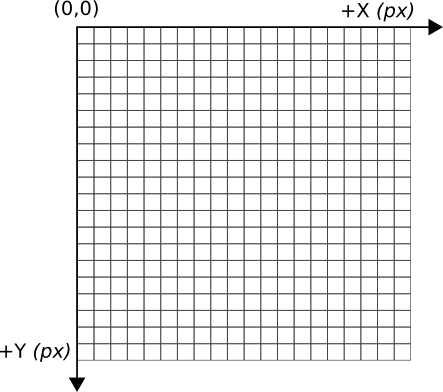
\includegraphics[width = 0.65\textwidth]{imgs/grid2d.png}
\end{center}

Tato konvence je převzata ze standartu počítačové grafiky, kdy první pixel v levém horním rohu nese souřadnicovou hodnotu právě {\em X = 0}, {\em Y = 0}. Obrácená osa Y se může ze začátku jevit matoucí. Důvody pro zdánlivé převrácení os pochopíme později například právě při operacích se samotnými obrazovými body, pixely, které jsou standartně uspořádány od levého horního rohu doprava a níže.

Plochu je možné představit si jako prázdný prostor, na kterém je možno zobrazovat grafiku. Tvary nebo například text se zobrazují právě prostřednictvím zdrojového kódu tj. instrukcemi psanými v editoru.

Na první pohled by se mohlo zdát, že například při zobrazení obdélníku, příkaz:

\begin{lstlisting}
rect(x,y,šířka,výška);
\end{lstlisting}

jehož výsledkem je kresba pouhého obdélníku je zbytečně komplikovaný, oproti jiným zobrazovacím metodám. Důležité je si zde uvědomit koncepci Processingu, který tímto zobrazením primitivních objektů sestavuje celý obraz. To co se zpočátku může zdát jako nadbytečná práce, tj. psaním koordinátů každého ze zobrazovaných objektů se posléze ukáže jako sofistikovaný a velmi ulehčující způsob přemýšlení o obraze. Veškeré parametry oddělené čárkou v kulatých závorkách příkazu {\em rect} náleží samotným vstupním hodnotám. Příkaz {\em rect} očekává čtyři parametry. Parametry mohou být celá čísla nebo čísla s desetinnou čárkou. Pro názornost, zadáme-li do parametrů ''natvrdo'' hodnoty:

\begin{lstlisting}
rect(8,6,7,5);
\end{lstlisting}

Výsledné zobrazení na naší pomyslné ploše bude následující:

\begin{center}
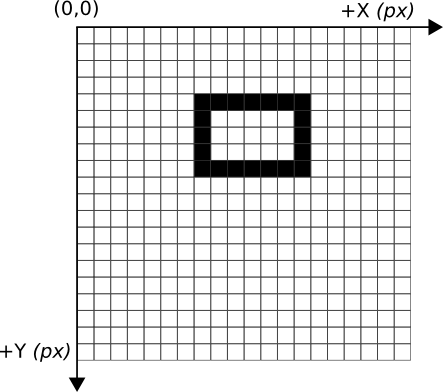
\includegraphics[width = 0.65\textwidth]{imgs/gridRect2d.png}
\end{center}


Zamyslíme-li se například o tom, že bychom v jakémkoli jiném nástroji chtěli zobrazit vícero, například tisíc obdélníků, na první pohled jednodušší GUI \footnote{zkratka pro "Guided User Interface" klasické grafické editory jako Gimp nebo Photoshop} grafické editory nám nedovolí tuto operaci učinit jinak, než že musíme všech tisíc obdélníků nakreslit. V případě Processingu nám bude stačit vytvořit rutinu pro kreslení libovolného počtu obdélníků a pak tuto rutinu spustit.

Zde se již dostáváme k samotnému jádru Processingového přemýšlení. Programování obecně dokáže velmi ulehčit operace jejichž pravidelnost dokážeme popsat. Veškeré umění psaní programu tedy spočívá v definicích těchto chování a redukci složitých jevů na jednoduché rovnice.

Celé řemeslné umění psaní kódu v podstatě záleží na eleganci v zápisu složitějších vztahů mezi různými parametry. Dovednosti se člověk učí postupně, osvojení si gramatické korektnosti a logické posloupnosti se mohou zpočátku jevit zbytečně komplikované, ovšem i po ovládnutí pouhých pár jednoduchých pravidel lze Processing využít kreativním způsobem.

V další části se budeme zabývat stavbou programu. Pod odpudivým názvem se skrývají právě tato jednoduchá pravidla, která by měla tvořit základ dalším experimentům. \bublina{zkuste si na kus papíru, nejlépe čtverečkovaného nakreslit jednotlivé objekty, uvědomte si v jakých dimenzích se pohybují}


\oddil{Hodnota a její zobrazení}

K čemu jsou vlastně hodnoty dobré? Tisk do konzole je jen kontrolní mechanismus většinou se nejedná o výslednou podobu programu.

Po celou dobu sčítání a odčítání hodnot jsme nezavolali žádnou funkci, která by kreslila na plátno.

Nyní je na čase ukázat si jakým způsobem Processing rozumí kresbě. Ty samé hodnoty které máme nyní v paměti mohou být použity pro jakýkoli kreslící výstup. Řekněme že chceme z těchto hodnot zobrazit například elipsu. K tomu potřebujeme zavolat funkci pro tvorbu elipsy, pokud ji nechceme zrovna z nějakých důvodů popisovat matematicky (to je samozřejmě dokonale možné).

Processing nemá předdefinované žádné složité tvary. Pracuje sám o sobě pouze s tvary primitivními, jako je bod, linka, trojúhelník, obdélník a elipsa. Pomocí těchto tvarů lze zkonstruovat nepřeberné množství obrazů. Představíme-li si nyní digitálně zpracovanou fotografii, můžeme například říci že je zkonstruována z bodů. Jednotlivé body, tj. pixely mají jinou barevnou hodnotu a takto poskládaný obraz se ve výsledku jeví jako fotografie.

Problém v případě konstrukce syntetické fotografie nespočívá v geometrii; ta je známa, mřížka bodů s počtem šířky krát výšky obrazových bodů digitální fotografie. Problém je v barevných hodnotách, které neznáme a synteticky jakoukoli matematickou funkcí těžko obsáhneme.

Dat pro výpočet fotorealistického obrazu potřebujeme opravdu hodně, nástroje které dokáží simulovat fotorealistický obraz existují a není jich málo. Dokonce i v Processingu existují podobné rozšíření které buď přímo zpracovává jí a zajištují obrazový výstup.

Tento příklad je trochu extrémní, ale naprosto pravdivý. Věc kterou se snažím ilustrovat je ta, že i s minimálním počtem primitivních geometrických tvarů lze docílit téměř nekonečné (spočitatelně obrovské) množství obrazů, což by nám mělo nadlouho stačit.

Nyní zpět k hodnotám. Máme-li již jakékoli hodnoty v paměti programu, můžeme kterékoli z nich namapovat na jakoukoli kreslící funkci. Zde začíná naše experimentální část, často se totiž stává, že výsledek kreslení neumíme plně předpovědět a teprve zobrazením nám kresba vzhledem k hodnotě začne dávat smysl.

Processing je, co se týče grafického výstupu, navržen pro přímou experimentální interakci vznikajícího programu s uživatelem. To znamená, že pokaždé kdy chcete vidět výsledek kódu, stačí pouze stisknout tlačítko {\em RUN}. Zpětná vazba spolu s vaší interpretací a úmyslem má potom veliký vliv na následné úpravy v kódu. Tímto způsobem můžete řekněme "vysochat" výslednou podobu programu.

\oddil{Kresba}

Jak zobrazit hodnoty, které uchovává program v paměti? Jakákoli hodnota lze použít například jako jeden z argumentů v kreslících funkcích.

Již zmiňovaný \vyraz{rect()}, tedy rectangle - obdélník, vyžaduje ke svému úspěšnému vykreslení čtyři parametry, čtyři číselné hodnoty \footnote{zde nezáleží jestli se jedná o celé číslo int nebo číslo s desetinnou čárkou float}. Tyto parametry, hodnoty, můžeme buďto zadat jako přímé číselné hodnoty, nebo do těchto parametrů můžeme zadat naši proměnnou která obsahuje číslo. Názorně:

\begin{lstlisting}

// první způsob vykreslení obdéníku
rect(10, 8, 40, 20);

// druhý způsob vykreslení obdélníku
int prvniCislo = 10;
int druheCislo = 8;

rect(prvniCislo, druheCislo, 40, 20);

\end{lstlisting}


\begin{center}
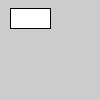
\includegraphics[width = 0.2\textwidth]{imgs/kresba-1.png}
\end{center}

Již nyní je nám zřejmé jak hodnoty mohou ovlivnit zobrazení. Namísto hodnot zadaných číselně se zde v druhém způsobu vykreslení obdélníku objevují naše proměnné, které mají již zadaný obsah. Výsledek zobrazení bude v obou případech stejný, ovšem z hlediska struktury programu je druhý způsob daleko flexibilnější.


V Processingu je předefinovaných jen několik základních tvarů, se kterými lze bohatě vystačit. Kromě již zmíněného \vyraz{rect()}, jsou zde také základní tvary:

\begin{itemize}
\item[\vyraz{point()}] - bod(x, y)
\item[\vyraz{line()}] - čára(x1, y1, x2, y2)
\item[\vyraz{ellipse()}] - elipsa(x, y, šířka, výška)
\item[\vyraz{triangle()}] - trojúhelník(x1, y1, x2, y2, x3, y3)
\item[\vyraz{quad()}] - čtyřúhelník(x1, y1, x2, y2, x3, y3, x4, y4) 

\end{itemize} \bublina{nakreslete jeden bod, čáru a elipsu tak aby se vzájemně nepřekrývali, zkuste změnit jejich pořadí sledujte změny po spuštění}

\pododdil{Výplň a obrys}

Některé tvary mají výplň a jiné (\vyraz{point()} a \vyraz{line()}) mají pouze konturu. Potřebujeme-li změnit barvu kresby objektů nyní můžeme použít vědomosti z předchozí kapitoly \odkaz{Barva}.

Výplň je definována jednou barevnou hodnotou přidanou do funkce \vyraz{fill()}. V kódu bude zápis vypadat následovně:

\begin{lstlisting}
fill(255,127,0);
rect(10, 10, 40, 20);

fill(0,127,255);
rect(10, 40, 40, 20);

\end{lstlisting}


\begin{center}
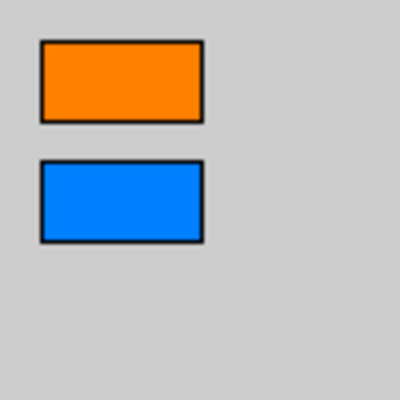
\includegraphics[width = 0.2\textwidth]{imgs/vypln-1.png}
\end{center}

Opak příkazu \vyraz{fill()} je \vyraz{noFill()}. Potřebujeme-li vykreslovat u objektů s výplní pouze jejich konturu můžeme použít právě příkaz \vyraz{noFill()}.

K ovládání barvy kontury použijeme příkaz \vyraz{stroke()}, ten opět přijímá hodnotu barvy. Jeho opakem je \vyraz{noStroke()}.

Ukažme si názorně zápisy:

\begin{lstlisting}
fill(255,127,0);
noStroke();
rect(10, 10, 40, 20);

noFill();
stroke(0,127,255);
rect(10, 40, 40, 20);

noFill();
stroke(0,127,255);
triangle(80, 70, 60, 60, 90,30);


stroke(255);
line(10,80,90,90);

\end{lstlisting}

Všimněte si zde pořadí v jakém příkazy určují výsledný obraz. Jeden příkaz na změnu barvy bude aplikován postupně na všechny objekty, které poté budou vykresleny, dokud nezměníte opět nastavení barev pro kresbu.

Výsledek kódu vypadá následovně:

\begin{center}

\includegraphics[width = 0.2\textwidth]{imgs/vypln-2.png}
\end{center}




Představme si nyní, že hodnota zadaná prvním způsobem zápisu se již nikdy v průběhu programu nemůže proměnit. V případě druhého způsobu zápisu získáváme díky možnosti změny jednoho parametru kontrolu nad kreslícím výstupem.

Veškeré příkazy, které jsme si zatím ukázali byli spuštěny pouze jednou. To znamená, že obdélník byl vykreslen a program, který již neměl žádné další příkazy jednoduše skončil.

V další kapitole si předvedeme jak vdechnout procesům pohyb a stálost, další kapitola je věnovaná animaci.



\oddil{Pohyb}

\pododdil{Proměnlivost}


Potřebujeme-li programu vdechnout život, musíme nejprve pochopit jakým způsobem se program může proměňovat.

Proměnlivost se dotýká základní myšlenky programu trvajícího v čase. K tomu abychom takovou proměnlivost mohli okem pozorovat, program může komunikovat pomocí různých výstupů. Processing, který byl navržen s důrazem na vizuální výstup, bude nejčastěji komunikovat právě vizuálně. Obecně řečeno proměnlivost je jakákoli změna hodnot v délce běhu programu, lze si ji představit například jako rozdíl mezi dvěma okénky filmu.

U filmových okének je rozdíl sice velmi těžko definovatelný, ilustruje ovšem dobře celý problém. Film nám spostředkovává iluzi pohybu sledem několika okének za vteřinu. Přesně stejně se chová i vizuální program. Rozdíl mezi filmem a programem je zhruba ten, že program může mít teoreticky dva a více různých konců, nebo nemusí končit vůbec. Zde by se dalo namítnout že program je také nakonec nositelem kauzálního sledu operací. Vtip je v tom, že stejný program spuštěný dvakrát nemusí produkovat stejný výsledek.

Změny v chodu programu se dá docílit několika způsoby. Základní změna v běhu programu je lidská intervence, která je z pohledu programu (respektive tvůrce programu) jen velmi těžko předpovídatelná. Změna v chování programu bez takového vnějšího zásahu je pak vždy umělá. (viz náhodnost)


Vraťme se ovšem k Proměnlivosti. Proměnlivost je nezbytnou součástí animace. Pohyb je proměna stavu v čase. Měli bychom zde mít vždy na paměti, že program nerozumí tomu co zrovna zobrazuje, program rozumí pouze hodnotám. Rozpohybovat lze tyto hodnoty, a tím posléze například jevy, které se v programu zobrazují a člověku dají nějaký smysl. 

Pro příklad si můžeme ukázat jak proměna jedné hodnoty ovlivňuje obraz. K tomu abychom mohli hodnotu proměňovat musíme ji nejdříve pojmenovat.

\begin{lstlisting}
int y = 0;
\end{lstlisting}

Tímto jsme pojmenovali svoji proměnnou. Jednou z možných variant zápisu je okamžité přiřazení hodnoty, tedy y je nyní nula. Pro animaci hodnoty použijeme přírůstek, tedy při kresbě jednotlivého okénka přičteme k hodnotě 1. Abychom viděli nějaký výsledek, můžeme opět kreslit objekt, který bude využívat proměňující se hodnotu v čase.

\begin{lstlisting}
void setup(){
	size(640,480);
}

void draw(){
	background(255);
	
	// prirustek o jedna
	// lze zapsat i zkracene y++;
	y += 1;
	
	// kresba
	line( 0 , y , width , y );

}
\end{lstlisting}

Po spuštění tohoto programu uvidíte animaci trvající 480 okének. Animace bude pokračovat i nadále, hodnota y se bude stále proměňovat. Kresba bude teoreticky probíhat mimo plátno. K tomu abychom kresbu udrželi v mezích plátna, můžeme použít jednoduchou podmínku, která bude vracet hodnotu y zpět na nulu.


\begin{lstlisting}
if(y > height){
	y = 0;
}
\end{lstlisting}

Celá tato procedura jen ilustruje logiku programu. Hodnota y je zde přímo zobrazena, ale stejně tak se dá použít kdekoli jinde, tedy ne nezbytně na kresbu. Pro lepší představu jiného použití uvedu následující příklad.

Pod hodnotou si lze například představit pevně stanovenou hodnotu, dejme tomu výšku domu. Zadání výšky nemusí nepostaví dům ale stanoví hodnotu se kterou můžeme dál počítat. Známe-li výšku plánované budovy, můžeme například přidávat patra dokud se této výšky nedosáhne. Tento postup již lze považovat za logickou konstrukci a jedním ze základních postupů jak takové logiky v programu docílit je podmínka. \odkaz{Podmínka} \bublina{vyzkoušejte podmínku na konec programu přidat a pak ji odstranit, ujistěte se že rozumíte tomu co v animaci způsobuje, změňte číslo v podmínce za jiné}

\pododdil{Animace}

Statická kresba na plátno je jen jeden z možných výstupů. Animace v Processingu znamená překreslovat plátno pokaždé jinými obrazy. Processing je jazyk využívaný zjeména v pohyblivém obraze. Nyní si ukážeme základní postup při tvorbě pohyblivého obrazu.


Jak jsme si již uvedli dříve \odkaz{Základní struktura programu} funkce \vyraz{draw()} je pouze prostředek pro změnu, nepřináší změnu sama o sobě. Funkce \vyraz{draw()} zajišťuje sousledné volání příkazů v neustálém trvání\footnote{po dobu běhu programu}. V Processingu si v podstatě uvědomíme, že psaním příkazů do smyčky píšeme pravidla jakoby pro jedno okénko ve filmu. Pohyb je vždy zajištěn proměnou našich datatypů \odkaz{Základní datatypy}, které v tomto okénku figurují.

Tedy například napíšeme-li takto, samotnou smyčku:

\begin{lstlisting}
void draw(){
	// 60x za vteřinu spuštěná operace
}
\end{lstlisting}

Vše uzavřeno do složených závorek bude spuštěno šedesátkrát za vteřinu. Bude-li obsah základní funkce \vyraz{draw()} neměnný, tj. budeme-li volat šedesátkrát za vteřinu to samé, animace bude ovšem v případě vizuálního výstupu jen abstraktním pojmem.

V tomto příkladě již dochází ke spuštění smyčky. Výsledkem bude pouze šedivá plocha v rozměrech sto krát sto pixelů, jelikož na plátno nebylo zatím nic vykresleno. Následujícími příkazy \vyraz{background()} a \vyraz{rect()} nakreslíme nejprve plné pozadí a následovně obdélník. Zápis bude vypadat následovně:

\begin{lstlisting}
void draw(){
	background(255);
	rect(10 , 10 , 30 , 30);
}
\end{lstlisting}

Takový zápis již provádí animaci a kreslí na plátno. Animace ovšem v tomto případě nebude patrná jelikož zatím se v obraze nic neproměňuje. Veškeré hodnoty jsou statické, tudíž se vykresluje jeden čtverec na bílém pozadí na stále stejném místě.

K rozhýbání objektů jednoduše potřebujeme proměnit jeden z parametrů v čase.\bublina{Animace je proměna obrazu v čase, jednotlivá okénka se v čase musí lišit. Přemýšlejte jakým způsobem k proměně může dojít.}  Abychom docílili animace zkusme například vložit namísto parametru pro kresbu čtverce v ose X počítadlo okének. Processing má již nastavenou proměnnou s údajem o počtu uběhlých okének pod názvem \vyraz{frameCount}.

Proměnnou \vyraz{frameCount} lze využít následovně:

\begin{lstlisting}
void setup(){
	size(640,480);
}


void draw(){
	background(255);
	rect( frameCount % width , 10 , 30 , 30 );
}

\end{lstlisting}

Výsledkem tohoto zápisu bude již první animace. Čtverec se bude pohybovat rychlostí šedesáti pixelů za vteřinu z leva do prava. Tato hodnota v podstatě udává počet vykreslených cyklů funkce \vyraz{draw()}, ta je v tomto případě pouze využita k pohybu vykreslovaného čtverce.

Počet okének vykreslovaných za vteřinu můžeme ovlivnit pomocí funkce \vyraz{frameRate()} vložené do funkce \vyraz{setup()}.

Tento pohyb je velmi názorný ukazuje, že hodnota počtu vykreslených okének lze použít například i jako hodnotu pro animaci. Stejně tak si můžeme založit i vlastní proměnnou, která bude mít identickou funkci.\footnote{v tomto konkrétním příkladě to sice nedává smysl, dá se použít stejně tak standartní proměnná \vyraz{frameCount}, příklad je zde jen pro ilustraci možností využití proměnných}

\begin{lstlisting}
// naše proměnná nazvaná příznačne: počítadlo
int pocitadlo = 0;


void setup(){
	size(640,480);
	frameRate(30);
}

void draw(){
	background(0);
	rect( pocitadlo, 10 , 30 , 30 );

	// zde již přičíáme hodnotu, lze napsat i zkrácným zápisem:
	// pocitadlo++;

	pocitadlo += 1;

	// zde můžeme použít modulo na omezení počítadla na šířku plátna

	pocitadlo = pocitadlo % width;

}

\end{lstlisting}

Definicí této hodnoty lze například časovat animace. Další metodou je animaci časovat pomocí funkce \vyraz{millis()}. Tato funkce je nezávislá na počtu vykreslených okének za vteřinu, měří počet uběhnutých milivteřin od startu programu. Může se nám také hodit pro precizní časování událostí v programu.


\pododdil{Dynamika pohybu}

K docílení jednoduché interakce není zapotřebí mnoho. Animace je ovšem složitější problém, který budeme řešit v Processingu nejvíce matematicky. Zdá se, že dosažení dynamického pohybu je jeden z průvodních jevů pokročilého programování.

 Nyní si můžeme ukázat jak lze zkombinovat dosavadní znalosti k vytvoření nelineárního pohybu.
 
 \begin{lstlisting}
float x;
float y;
float rychlost;

void setup(){
	size(640,480);
     x = width / 2;
     y = height / 2;
     rychlost = 0.1;
}

void draw(){
	background(255);
	x += (mouseX - x) * rychlost;
	y += (mouseY - y) * rychlost;
	rect(x,y,30,30);
}
\end{lstlisting}

Čtverec bude nyní následovat kurzor nelineárním pohybem. Dynamika pohybu je dána prostou formulí:
\begin{lstlisting}
x += (mouseX - x) * rychlost;
y += (mouseY - y) * rychlost; 
\end{lstlisting}\bublina{opište formuli a zkuste změnit rychlost, pozorujte změny, změňte hodnoty tak, aby se objekt pohyboval po křivce}
K proměnným {\em x} a {\em y} přiřazujeme zlomek rozdílu mezi pozicí kurzoru a proměnou v obou osách. Tuto formuli lze využít téměř kdekoli, například při jemném přechodu barev a vyhlazování hodnot obecně.

Druhá proměnná {\em rychlost} by se k docílení podobného efektu měla pohybovat v rozmezí od 0 do 1.




\oddil{Podmínka}

Uvedením do stavů programu se můžeme dostat k prvnímu opravdovému strukturování programu. Zkusme nyní nastínit, jak taková struktura vypadá. Patrně nejpřímější řízení dějů v programu je podmínka. Podmínka říká, jestliže je něco pravda, spusť následné příkazy. Podmínka funguje v podstatě jako výhybka, která odklání program do jeho různých cest. Uvedu zde krátký příklad vytváření podobné struktury v programu:

\begin{lstlisting}
boolean prepinac = false;
int hodnota;

if(prepinac == true){
    hodnota = 1;
}else{
    hodnota = 0;
}

println(hodnota);

\end{lstlisting}

Velmi prostá struktura je v tomto příkladě vytvořená jednou podmínkou. Podmínka je v Processingu (a řadě jiných jazyků) značena slovem \vyraz{if}, \uv{jestli}. \uv{Jestli} potřebuje dostat odpověd v kulatých závorkách, ta může být jen pravda nebo nepravda, k tomu se hodí nejlépe již zmíněný \vyraz{boolean}, nebo například porovnávání dvou čísel, znaků nebo řetězců znaků, tj. operace které nám vrátí \vyraz{true} nebo \vyraz{false}.

Definujeme-li tedy náš \vyraz{boolean} na začátku jako nepravdu, podmínka se v tomto případě nenaplní a program spustí kód uvozený složenými závorkami následujícími až slovo \vyraz{else}.

V našem příkladě se jedná o druhou větev podmínky, ta sice není povinná, ale pro ukázku jsem ji zde rovnou zmínil. Tedy za ukončením \vyraz{if} a složených závorek můžeme dále slovem \vyraz{else}, tzn. \uv{jestliže ne}, řící co se stane v případě nenaplnění naší podmínky.

V tomto konkrétním případě se k proměnné {\em hodnota} přiřadí číslo {\em 0}.

To program následně ověřuje tiskem do konzole, kde se objeví {\em 0} 


\pododdil{if}

Jak jsme si již uvedli, podmínka je jeden ze základních stavebních kamenů programu. Podmínku lze použít ve všech případech, kdy předpokládáme jednoznačnou odpověď {\em ano} nebo {\em ne}. Podmínka v Processingu, stejně tak jako ve většině ostatních jazyků, konstruována příkazem \vyraz{if}.

Konstrukce podmínky vypadá pak následnovně:


\begin{lstlisting}

boolean pravda = true;

if(pravda == true){

    // spust nasledujici blok

}

\end{lstlisting}

Za povšimnutí zde stojí dvojité rovnítko. Tento speciální symbol se používá při porovnávání dvou stran. Proměnná nazvaná {\em pravda} získala hodnotu \vyraz{true}. V případě podmínky nezáleží na počtu proměnných v kulatých závorkách, otázka může být i více kombinovaná záleží na výsledky, který vždy musí být pravda nebo nepravda, tedy \vyraz{true} nebo \vyraz{false}. Pro zkonstruování takové věty lze použít následující znaménka.\bublina{vyzkoušejte i jiné logické operace, ujistěte se, že správně rozumíte jak fungují, použijte vykřičník jako zápor, změňte logické operace}

\begin{lstlisting}
boolean pravda = true;
int cislo = 3;
String text = "Lorem ipsum dolor et amet";

if(cislo == 3){
    // tato podminka je spustena
}

if(cislo != 3){
    // tato podminka neni spustena, znamenko nerovna se je opakem rovnitka
}

if(cislo > 3){
    // tato podminka neni spustena cislo neni vetsi nez 3
}

if(cislo < 3){
    // tato podminka neni spustena cislo neni mensi nez 3
}

if(cislo >= 3){
    // tato podminka je spustena, znamenko vetsi nebo rovna se, cislo rovna se 3
}

if(cislo <= 3){
    // tato podminka je spustena, znamenko mensi nebo rovna se, cislo rovna se 3
}

if(text.equals("Lorem ipsum dolor et amet")){
	// tato podminka je spustena, porovnavani textu je take mozne, osem pozor
	// k porovnavani celych retezcu, textu se pouziva funkce equals("String")
}

\end{lstlisting}

Takovým výčtem operací jsme si pokryli základní konstrukci podmínky. Další znaménka slouží ke skládání jednotlivých otázek. Znaménko pro logicke A je:

\begin{lstlisting}
boolean a = true;
boolean b = false;

if(a == true && b == false){
	// tento blok bude spusten, a je pravda A b je pravda
}

if(a == true && b == true){
	// tento blok nebude spusten, b totiz neni pravda, b == false
}

\end{lstlisting}


("appersand" se na české klávesnici nevyskytuje, na anglické klávesnici jej naleznete většinou pod \klavesy {SHIFT - 7}), pro logické NEBO se používá dvojitá svislá čára tzv. pipe:

\begin{lstlisting}
boolean a = true;
boolean b = false;

if(a == true || b == false){

	// tento blok bude spusten, k tomu staci pouze ze a je pravda NEBO b je pravda

}


if(a == true || b == true){

	// tento blok bude tedy opet spusten

}


if(a == false || b == true){

	// tento blok jiz spusten nebude, ani a ani b neni pravda 

}

\end{lstlisting}

Za pomoci skládání otázek můžeme zkonstruovat celé věty a složitější otázky. V kombinaci s kulatými závorkami si vystačíme pouze s logickým AND a OR. Zkusme si ilustrovat situaci následovně:


\begin{lstlisting}
boolean a = true;
boolean b = true;
boolean c = false;

if( (a && b) || c ){

	// tento blok bude spuštěn
	
}

if( !(a && b) || c ){

	// tento blok nebude spuštěn
	
}

\end{lstlisting}

Jaký je rozdíl mezi prvním a druhým blokem? Poslední specialita booleanovských operací je znaménko vykřičník. Takové znaménko před proměnou typu \vyraz{boolean} znamená opak tvrzení tedy, je li {\em pravda} pravdou, {\em !pravda} \label{!pravda} je nepravdou tedy výsledkem je \vyraz{false}.\bublina{zkuste si v duchu představit otázky na které lze odpovědět ano nebo ne, zkuste je poté přepsat do tvaru podmínky, zkuste k tomu využít další proměnné porovnávejte je a pokuste se přemýšlet k čemu se dají takto využít}


\begin{lstlisting}
boolean pravda = true;

println( pravda ); // tiskne true
println( !pravda ); // tiskne false
\end{lstlisting}



Dále si všiměte, že v podmínce chybí jakékoli porovnávací znaménko. Ve skutečném programování se setkáte spíše s tímto zápisem, je to zápis zkrácený. Namísto neustálého rozepisování {\em něco rovná se rovná se \vyraz{true}} lze napsat pouze v kulatých závorkách. Je-li naše {\em něco} datového typu \vyraz{boolean} Processing bude takovému zápisu rozumět. Tedy nejjednodušší zápis může vypadat i takto:

  
\begin{lstlisting}
boolean a = true;

if(a)
	//pouze tento jediný řádek bude spuštěn
	
	
if(a){
	// cely tento blok
	// bude spusten
}
\end{lstlisting}

K úplnému zkrácení se dají i vypustit i složené závorky, to vede opět k rychlejšímu zápisu. Rozdílem takového zápisu je fakt, že taková podmínka spouští pouze jeden následující řádek. Přestože je to naprosto správný způsob programování, někteří programátoři takový zápis neradi používají z důvodu zhoršení přehlednosti v kódu. Opět se s takovým zápisem často setkáte, člověk je jednoduše líný živočišný druh a \vyraz{if} se v programování používá opravdu často.

\pododdil{else}

K dalšímu rozšíření podmínek slouží příkaz \vyraz{else} a dá se přeložit takto. Jestliže je něco pravda udělej toto, jestliže ne udělej něco jiného. Zápis vypadá takto:

\begin{lstlisting}
boolean a = false;

if(a){

	// kdyby a bylo true, tak bu se spustil tento blok kodu 

}else{

	// ale protoze je nase a false, spusti se nyni kod
	// v tomto bloku
	
}
\end{lstlisting}



\pododdil{ ? : }

Abychom podmínky vyčerpali nadobro ukážeme si poslední možný zápis, který je ještě úspornější. \bublina{vyzkoušejte si zkrácené zápisy, ověřujte jejich funkčnost tiskem do konsole nebo například proměnou barev objektů}
  
  
\begin{lstlisting}
boolean a = true;

if(a)
	background(0);
	
	
background( a ? 0 : 255 );

\end{lstlisting}






\oddil{Interakce}

\Slovnik{interakce} se dá obecně definovat jako vzájemné působení. V počítačové terminologii se nejvíce má na mysli vzájemné působení člověka a stroje. Přímá interakce z podstaty vzájemného působení vyžaduje rozměr času animaci\footnote{tedy program trvající v čase}. To umožňuje uživateli přímý vstup do proměnných, tedy do obsahu našich hodnot.

Je dobré si uvědomit, že \slovnik{interakce} je do jisté míry při práci s počítačem pozorovatelná neustále. Pouhý pohyb myši lze považovat za interakci člověka se strojem. Pohyb uživatele přímo proměňuje hodnoty vykreslující pozici kurzoru, stiskem klávesy v textovém editoru například píšeme text atd.

Při interakci je nutné do určité míry předvídat chování uživatele. Interakce primárně vychází z fyzické zkušenosti s předměty kolem nás. Interakcí je myšleno vše co může uživatel přímo ovlivnit.

Interakce se dá rozdělit do dvou základních oblastí na interakci přímou a nepřímou, nebo chcete-li na interakci vědomou a nevědomou. Mezi těmito kategoriemi neexistuje jednoznačná hranice.

Obecně je toto rozlišení spíše stupnicí od jednoduchých přímo a okamžitě viditelných jevů po uživatelově vstupu ke komplikovanějším procedurám spouštěným jen s částečným vědomím uživatele.

Základní tedy přímou interakci si můžeme ukázat na následujícím příkladě:

\begin{lstlisting}
void setup(){
	size(640,480);
}

void draw(){
	background(0);
	// vsimnete si parametru mouseX a mouseY
	rect(mouseX,mouseY,30,30);
}
\end{lstlisting}


\vfill
\begin{center}
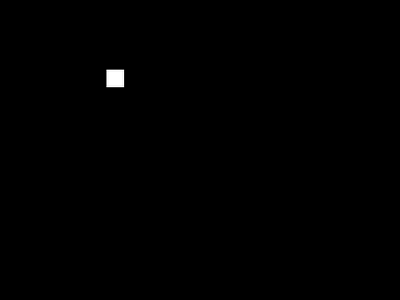
\includegraphics[width = 0.8\textwidth]{imgs/interakce-1.png}
\end{center}

Toto je jedna z nejzákladnějších možných interakcí. Vstupem pro pozici kresleného obdélníku se nám stávají dva parametry \vyraz{mouseX} a \vyraz{mouseY}.

Čtení pozice myši je jedním nejsnazších možných způsobů interakce stroje z člověkem. Nyní si ukážeme jak lze detekovat stisknutí tlačítka myši. Pro tento účel můžeme využít předdefinovaných metod Processingu. K detekci kliku lze použít funkci \vyraz{mousePressed()}.


\begin{lstlisting}
boolean stisknuto = false;

void setup(){
	size(640,480);
}

void draw(){
	background(0);
	
	if(stisknuto){
		fill(255);
	}else{
		fill(255,0,0);
	}
	
	rect(mouseX,mouseY,30,30);
}

void mousePressed(){
	stisknuto = !stisknuto;
}

\end{lstlisting}


\begin{center}
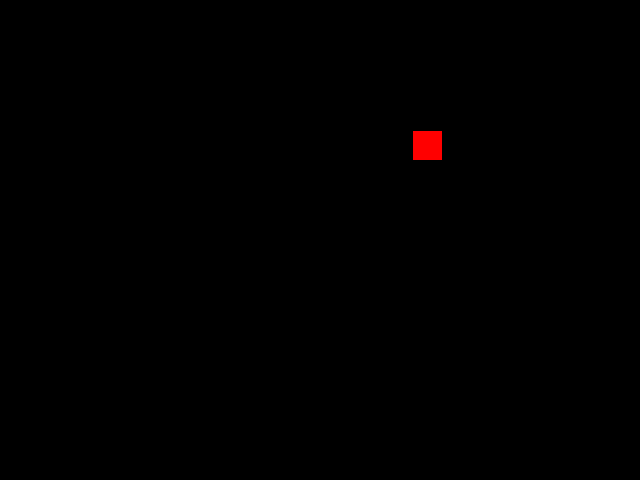
\includegraphics[width = 0.8\textwidth]{imgs/interakce-2.png}
\end{center}

Všimněte si poslední funkce. (Více o funkcích obecně v \odkaz{Funkce}) Ta je programem spuštěna jen tehdy stiskne-li uživatel tlačítko myši. Abychom uchovali informaci o stisku přepneme jím stav jedné z našich proměnných nazvané {\em stisknuto}. Jednořádkový zápis s vykřičníkem je zkrácení pro přepnutí stavu. \odkaz{Podmínka}

K tomu abychom detekovali stisk tlačítak myši použijeme funkci \vyraz{mousePressed()}. Další možnosti interakce jsou detekovat které tlačítko myši jsme stiskli, popřípadě detekovat stisk klávesy. Výčet dalších možností je následující:


\begin{lstlisting}
// detekce stisku tri ruznych tlacitek mysi
void mousePressed(){
	if(mouseButton==LEFT){
	
	}else if(mouseButton==RIGHT){
	
	}else if(mouseButton==CENTER){
	
	}
}


// detekce tazeni stisknute mysi
void mouseDragged(){
	// muzeme zde opet detekovat tlacitko
}

// timto detekujeme moment
// uvolneni stisku tlacitka
void mouseReleased(){
	// opet zde muzeme detekovat ktere
	// tlacitko bylo stisknuto
}

// stisk klavesy s detekci typu
void keyPressed(){

	if(key=='a'){
	
	}else if(keyCode=='ENTER'){
	
	}
}

// opet detekce uvolneni klavesy
void keyReleased(){

}

\end{lstlisting}

Tímto výčtem jsme pomalu vyčerpali možnosti interakce se standartními vstupy uživatele v Processingu. Veškeré tyto definice musí stát mimo základní funkce Processingu, tedy mimo \vyraz{setup()} a \vyraz{draw()}.

Proměnná \vyraz{mouseButton} nám říká údaj o naposledy stisknutém tlačítku myši, stejně tak funguje proměnná \vyraz{key} a \vyraz{keyCode} ve funkci \vyraz{keyPressed()} a \vyraz{keyReleased()}.

Obě proměnné \vyraz{key} a \vyraz{keyCode} mohou mít buď číselnou reprezentaci, kterou lze vyhledat v mapě znaků, nebo v případě se dají porovnávat s pojmenovanými klávesami v processingu.

Jestliže je klávesa kódovaná zjistíme dále pomocí proměné \vyraz{CODED}. Asi takto:

\begin{lstlisting}
void keyPressed(){

	if(CODED){
		if(keyCode=='ENTER'){
			// detekce klavesy ENTER
		}
	}else{
		if(key==' '){
			// detekce mezerniku
			// porovnano s prazdnym znakem
		}
	}
}
\end{lstlisting}

Hrubý výčet pojmenovaných kláves, které můžeme porovnat s proměnnou \vyraz{keyCode} je následující:

\begin{lstlisting}
// spiky
UP, DOWN, LEFT, RIGHT

// specialni klavesy
ALT, CONTROL, SHIFT

// dalsi dulezite klavesy
BACKSPACE, TAB, ENTER, RETURN, ESC, DELETE
\end{lstlisting}

Nevime-li si rady jak určitou klávesu detekovat. Můžeme si jednoduše vytisknout do konzole její číslo pomocí  příkazu \vyraz{println()}.


\begin{lstlisting}
void keyPressed(){
	println("cislo klavesy: "+key);
}
\end{lstlisting}

\bublina{vyzkoušejte detekovat různé klávesy, zkostruujte jendoduché přepínače které mohou reagovat na podněty}


\oddil{Pole}

Jedna proměnná může uchovat pouze jednu hodnotu. V programování se brzy dostaneme do situace, kdy budeme potřebovat operovat s vícero hodnotami najednou. Tak například cheme-li použít deset čísel z fibonacciho řady můžete si je definovat postupně.

\begin{lstlisting}
int hodnota0 = 2;
int hodnota1 = 3;
int hodnota2 = 5;
int hodnota3 = 8;
int hodnota4 = 13;
int hodnota5 = 21;
int hodnota6 = 33;
int hodnota7 = 54;
int hodnota8 = 87;
int hodnota9 = 141;
\end{lstlisting}


Ke zkrácení zápisu, namísto neustálého přepisování téhož je zde takzvané pole. Pole neboli {\em Array} se v programování vyznačuje hranatými závorkami.

\begin{lstlisting}
int mojePoleHodnot[];
\end{lstlisting}

Všimněte si zde pouze hranatých závorek na konci názvu proměnné. Druhý možný zápis s naprosto identickým významem je vložit hranaté závorky před název definované proměnné.


\begin{lstlisting}
int [] mojePoleHodnot;
\end{lstlisting}

Oba způsoby jsou naprosto identické. Pouhá definice pole ovšem pole nevytváří. K tomu abychom nyní do pole něco mohli začít ukládat, musíme ho nejprve inicializovat na pevný počet hodnot. V tomto případě lze buď hodnoty zadat přímo v definici pole. Pro takovou operaci lze využít zápis pomocí složených závorek:

\begin{lstlisting}
int mojePoleHodnot[] = {0,1,1,2,3,5,8,13,21,33};
\end{lstlisting}

Tento zápis inicializace je v tomto konkrétním případě zřejmě nejrychlejší. Hodnoty z pole, které je nyní celé uloženo pod jednou proměnnou můžeme získat následujícím způsobem:

\begin{lstlisting}
int mojePoleHodnot[] = {0,1,1,2,3,5,8,13,21,33};

println(mojePoleHodnot[0]);
println(mojePoleHodnot[1]);
println(mojePoleHodnot[5]);
//atd.
\end{lstlisting}


Další způsob zápisu je ovšem obvyklejší a jak se dozvíme v příští kapitole bude pro nás nejvýhodnější.


\begin{lstlisting}
int mojePoleHodnot[];

void setup(){
	mojePoleHodnot = new int[10];
	
	mojePoleHodnot[0] = 0;
	mojePoleHodnot[1] = 1;
	mojePoleHodnot[9] = 33;
	// atp.
}
\end{lstlisting}

Všimněte si že v zápisu se objevilo slovo \vyraz{new}. Toto slovo jsme zatím nepoužili a jeho význam rozvedeme později \odkaz{Třída a objekt}. K tomu abychom přiřadili hodnotu jednotlivých míst v poli, musíme nejdříve vepsat do hranatých závorek kam budeme zapisovat. Stejně tak se později k číslu, které jsme uložili, můžeme dostat. 

Tímto způsobem jsme si definovali pole o rozměru deseti hodnot. Stále je ovšem patrné že v kódu se zbytečně opakujeme rozepisováním názvu jedné proměnné.\bublina{Pole jsou abstraktní koncepce. Ujistěte se, že dobře rozumíte jakým způsobem pracují. Najděte si pro pole vhodnou paralelu, například číslované zásuvky pro představu fungují dobře, pročtěte si kapitolu klidně vícekrát, aby jste polím dobře rozuměli.}

Hodnot v polích nebude vždy jen deset. K lepší práci s poli potřebujeme rychlejší způsob, jak na to zjistíte v následující kapitole věnované smyčkám. 


\oddil{Smyčka}


Smyčka je mocný nástroj a dobrý pomocník při práci s opakovatelnými operacemi. V minulé kapitole jsme si definovali pole. Definici nyní zopakujeme a zkusíme ji více automatizovat pomocí smyčky.

\begin{lstlisting}
int mojePoleHodnot[];

void setup(){
	mojePoleHodnot = new int[10];
	
	for(int i = 0; i < 10; i += 1){
		mojePoleHodnot[i] = 0;
	}
}
\end{lstlisting}

A první smyčka je na světě. Zápis, který vypadá na první pohled trochu odpudivě může být váš dobrý přítel. Trochu si jej rozebereme. 

Formule začíná slovem \vyraz{for}. Následují kulaté závorky. V nich je v podstatě rozsah, který potřebujeme zopakovat. Hodnoty jsou odděleny středníkem. \bublina{vyzkoušejte si rozdílné smyčky s různým rozsahem, opakujte si složitější zápis for dokud ho nebudete umět sami bezchybně zkonstruovat, zkuste smyčku využít s měnící se proměnnou uvnitř, kreslete ze smyčky objekt}

\begin{itemize}
\item[počátek] int i = 0
\item[konec] i < 10
\item[přírůstek] i += 1
\end{itemize}

Hodnota, se kterou pracujeme, se jmenuje {\em i}, ale může se jmenovat dle vaší libosti například:

\begin{lstlisting}
	for(int pocitadlo = 0; pocitadlo < 10; pocitadlo += 1){
		mojePoleHodnot[pocitadlo] = 0;
	}
\end{lstlisting}

Dle potřeby lze také definovat rozsah smyčky. Například počítání v opačném pořadí.


\begin{lstlisting}
	for(int pocitadlo = 9; pocitadlo >= 0; pocitadlo -= 1){
		mojePoleHodnot[pocitadlo] = 0;
	}
\end{lstlisting}

Název pro jednoduchou smyčku {\em i} se používá velmi často, může například značit slovo {\em index}. Smyčky vykonávají v programu tvrdou práci, používají se na hromadné operace z nichž se často stávají náročné výpočty.

Vraťme se ovšem k definici {\em fibonacciho} řady z předchozí kapitoly. \odkaz{Pole}. Pokusíme se nyní skloubit to co jsme se naučili o \slovnik[smyčka]{smyčkách} a \slovnik[pole]{polích}. Zkusíme si napsat jednoduchý program, který nám vygeneruje tolik čísel z {\em fibonacciho řady} kolik budeme potřebovat.


\begin{lstlisting}
int delka = 20;
int fibonacci[];

void setup(){
	fibonacci = new int[delka];
	fibonacci[0] = 0;
	fibonacci[1] = 1;
	
	
	for(int i = 2; i < delka; i += 1){
		fibonacci[i] = fibonacci[i-1] + fibonacci[i-2];
	}
	
	println(fibonacci);
}

\end{lstlisting}

V konzoli se nám objeví.

\begin{lstlisting}
[0] 0
[1] 1
[2] 1
[3] 2
[4] 3
[5] 5
[6] 8
[7] 13
[8] 21
[9] 34
[10] 55
[11] 89
[12] 144
[13] 233
[14] 377
[15] 610
[16] 987
[17] 1597
[18] 2584
[19] 4181
\end{lstlisting}

Čísel samozřejmě může být nepočitatelně. Smyčky mají tu výhodu, že dokáží opakovat jednu operaci. Můžeme využít jazyka k definici operace a zapojením dalších proměnných ji povýšit na princip. Máme-li takto zpracovaný princip můžeme jej například zobrazit, nebo s ním díle pracovat. K dalšímu uspořádání se dostaneme v další kapitole \odkaz{Funkce}

Pro ilustraci fibonacciho řady můžeme využít druhou smyčku ke kresbě

\begin{lstlisting}
for(int i = 0; i < delka; i += 1){
	line(fibonacci[i],0,fibonacci[i],height);
}
\end{lstlisting}

A výsledkem bude:

\begin{center}

\includegraphics[width = 0.8\textwidth]{imgs/smycka-1.png}
\end{center}


\oddil{Uspořádání, stuktura programu}
\index{void}

Jednotlivé bloky kódu lze dále strukturovat. Strukturování v kódu se provádí zpravidla tam kde potřebujeme opakovaně spouštět identický blok kódu nebo si potřebujeme zpřehlednit probíhající operace.


\pododdil{Funkce}

Nejjednoduším řešením problému je jeho rozdělení na menší části. Problém jak dojít k jednomu výsledku se dá rozložit na jednotlivé po sobě jdoucí události a ty postupně popsat.

Dílčí operace si pro přehlednost můžeme definovat do bloku takzvané funkce. Základní funkcí je takzvaný \vyraz{void}. Void v podstatě tvoří blok kódu který je spuštěn jeho pozdějším zavoláním. Jestliže jednotlivé proměnné by ve větě mohli označovat podstatná jména funkce se dají chápat jako slovesa. S funkcemi jsme se setkali již dříve při definici základních smyček programu.

\begin{lstlisting}

void setup(){

}

void draw(){
	nakresliObdelnik();
}

void nakresliObdelnik(){
	rect(10,10,20,20);
}

\end{lstlisting}

Vedle standartních funkcí Processingu setup a draw jsme si nyní definovali třetí funkci nakresli obdélník. Tato funkce je pak spuštěna unitř kreslící smyčky draw.

V tomto konkrétním případě samotná funkce nedává mnoho smyslu. Příkaz rect v podstatě není nic jiného než-li funkcí processingu “nakresli odélník”. Všimněme si ovšem že tato funkce rect má v kulatých závorkách parametry, které označují kde má být obdélník vykreslen. Tyto parametry se v programování obecně nazývají arguments.

Chceme-li vytvořit funkci a potřebujeme-li do ní poslat vstupní parametry, můsíme při její definici vepsat do kulatých závorek jaké parametry bude funkce očekávat.


\begin{lstlisting}

void nakresliObdelnik(int x, int y){
	rect( x , y , 20 , 20 );
}

\end{lstlisting}

Jednotlivé parametry se v kulatých závorách oddělují čárkou a může jich být teoreticky neomezené množství.

Důležité je upozornit že vstupní hodnoty jsou vytvořeny pokaždé spustíme-li funkci a zanikají je-li funkce ukončena. Takovým proměným se říká dočasné. V programátorské praxi se můžeme setkat s jejich uvozovanim podtržítkem.


\begin{lstlisting}

void nakresliObdelnik( int _x, int _y ){
	rect( _x , _y , 20 , 20 );
}

\end{lstlisting}

Podtržítka nemají žádou funkci jsou jen součástí názvu proměnné a programátoři je používají pro lepší organizaci.

V processingu lze dále definovat funkce, které se jmenují stejně ale musí mít jinou skladbu vstupních hodnot. Představme si že budme potřebovat dvě funkce nakresliobdelnik, jednu můžeme nechat bez vstupních parametrů a druhou budeme definovat s parametry x a y. Tímto způsobem můžeme odlišit dvě různé funkce pouze způsobem spuštění.


\begin{lstlisting}

void nakresliObdelnik( int _x, int _y ){
	rect( _x , _y , 20 , 20 );
}

void nakresliObdelnik(){
	rect( 10 , 10 , 20 , 20 );
}

void draw(){
	nakresliObdelnik();
	nakresliObdelnik( 10 , 20 );
}

\end{lstlisting}

Tento příklad je správně a vykreslí dva různé obdélníky. Máme nyní na výběr potřebujeme-li zadat parametry nebo ne, v druhém případě se nakreslí obdélník v předem nadefinované pozici.


Void je pouze jedna z možností definic funkcí. Další mozné funkce můžeme definovat podle datatypů, které budeme očekávat za výsledek funkce. Tedy můžeme si definovat funkci, která nám zjistí zda-li se kurzor nachází v daném obdélníku. Namísto prázdného void budeme očekávat odpověď ve tvaru boolean pravdu nebo nepravdu. Funkce uvozená datatypem bude vždy očekávat odpověď ve stejném tvaru takového datatypu. Pomocí slova return můžeme funkci přiřknout výsledek, v tomto případě true nebo false.

\begin{lstlisting}

Void setup(){

	size(640,480);

}

void draw(){
	if( jeKurzorVObdelniku(10,20,20,20) ){
		nakresliOdelnik(10,20);
	}

}

boolean jeKurzorVObdelniku(int _x, int _y, int _sirka, int _vyska){
	
	if(mouseX >= _x && mouseX <= _x +_sirka &&
	mouseY >= _y && mouseY <= _y +_vyska){
	
		return true;
	
	}else{
	
		return false;
	
	}
}

void nakresliObdelnik(){
	rect( 10 , 10 , 20 , 20 );
}

void nakresliObdelnik(int _x, int _y){
	rect( _x , _y , 20 , 20 );
}

void nakresliObdelnik(int _x, int _y, int _sirka, int _vyska){
	rect( _x , _y , _sirka, _vyska );
}


\end{lstlisting}


Bude-li se kurzor nacházet v prostoru vymezeném v otázce, nakreslí se obdélník o stejné velikosti. Náš program již začíná být strukturovaný. Tímto způsobem můžeme dále větvit podmínky a rozdělovat kód do jednotlivých spustitelných bloků příkazů.

Funkce stejně jako proměnné doporučuji pojmenovávat stručně a výstižně. U funkcí dále platí, že by měli dělat pouze jednu věc a měli by ji dělat dobře. Je lepší problém rozdělit na více funkcí a tím  strukturovat program. Strukturování podobným způsobem je velmi výhodné budete-li se ke kódu vracet s odstupem času, nebo bude-li jej číst někdo jiný než vy.

Budete-li kód chtít sdílet, je dobré jej učinit co nejvíce čitelný pro druhé lidi. Ze je velmi dobrá tradice napsat ke každé funkci, jeden řádek nebo odstavec o tom co funkce přesně dělá  (u které to není na první pohled zřejmé).

Co se délky funkcí týče dobré pravidlo zní: Přesáhnete-li počet vnitřích proměnných tucet, měli by jste už přemýšlet o rozdělení do dvou funkcí.

\pododdil{Funkce a jejich datatypy}

Funkce \vyraz{void} je jen jednou možností z celé škály definic funkcí. Prázdná funkce \vyraz{void} nic nevrací zpět, jednoduše řečeno nemá žádný výsledek. Funkci s výsledkem můžeme definovat pomocí příkazu \vyraz{return} zevnitř funkce.

Příkaz \vyraz{return}, musí být stejného datatypu jako je naše funkce. Pro pochopení pudu lépe ilustrovat zápis plodné funkce. Řekněme že potřebujeme funkci, která k ke vstupní proměnné přičte polovinu její hodnoty. Taková funkce by mohla vypadat následovně:

\begin{lstlisting}
float prictipolovinuHodnoty(float _vstup){

	_vstup += _vstup / 2;
	return _vstup;

}

\end{lstlisting}

Za pozornost zde stojí namísto slova \vyraz{void}, nám již dobře známé slovo \vyraz{float}. Zapojen9 takov0 funkce do chodu na3eho programu by v praxi mohlo vypadat následoovně:
\begin{lstlisting}
float a = 5;

println(a);
// vytiskne 5 do konzole

a = prictipolovinuHodnoty(a);

println(a);
// vytiskne 7.5

a = prictipolovinuHodnoty(a);

println(a);
// vytiskne 11.25

//atd.
\end{lstlisting}

Jak můžeme vidět. Definice funkce zůstala stejná a výsledky se liší podle zaslaných argumentů, vstupních hodnot do funkce. Naše vlastní definice funkcí můžou mít dále jakékoli datatypy, které již známe.

\begin{lstlisting}

String pozdrav(){
	return "ahoj!";
}

int inverze(int _vstup){
	return vstup*(-1);
}

// vice moznosti podminkou

String pozdrav(int _vstup){
	if(_vstup==1){
		return "ahoj tisknu jedna!";
	}else if(_vstup==2){
		return "ahoj tu mate dva!";
	}else{
		return "Dobry den, nevim co chcete ...";
	}
}
// atd.

\end{lstlisting}
\bublina{zkuste si zvykat na strukturování pomocí funkcí, využívejte je všude kde vznikne ucelená operace, zkuste přemýšlet a definovat obecné a šikovné funkce, myslete na psaní komenářů u dlouhých funkcí, pomocí funkcí zkuste udržet draw() co nejpřehlednější}


V další kapitole se přesuneme defacto již k definici vlastních datatypů, budeme hovořit o třídách a objektech.





\pododdil{Třída a objekt}

Funkce jsou jeden způsob jakým můžeme strukturovat program. Veškerý kód, který jsme doposud psali je vlastněn takzvanou třídou. Třída vlastní veškeré funkce i proměnné, které v Processingu běžně píšeme. Můžeme to nazvat mateřským objektem. V rámci tohoto objektu můžeme definovat své vlastní objekty, které můžou mít různé vlastnosti.

V úvodu jsme se dozvěděli že Processing je objektově orientovaný jazyk. Nad tím je na čase se pozastavit. Co to vlastně znamená objekt. Ilustrace koncepce programování je prostá, stačí se rozhlédnout kolem sebe a zaměřit se na jeden konkrétní objekt (hrnek, propiska, kniha). Tento objekt má některé vlastnosti. Tak například propiska má svoji hmotnost, rozměry ve tří osách, barvu náplně, obsah náplně a barvu jako takovou, pravděpodobně také nějaké logo jako potisk. Tužka dále může být \uv{rozcvaknutá} nebo \uv{zacvaknutá}, mohli bychom takto pokračovat dále. Všechny tyto vlastnosti si můžeme představit jako naše proměnné. Třída pak bude to, co mají propisky společného, jednotlivými paremetry budeme odlišovat jednu propisku od od druhé.

To co s propiskou můžeme dělat si představme jako funkci. Tak například propisku můžeme \uv{rozcvaknout} a \uv{zacvknout}. Tužkou můžeme psát atp. Tyto činnosti ovlivňují naše parametry konkrétního objektu.

Třída je tedy souhrn definicí, které vyjadřují nějaký typ objektu, propisku, tužku, hrnek. Objekt je pak konkrétní kus propisky, hrnku atp.

V kódu naše propiska vypadá takto:


\begin{lstlisting}
class Propiska{

	// promenne hodnoty propisky
	float rozmery[];
	float pozice[];
	color barvaNaplne;
	boolean zacvaknuta;
	String napis;

	// konstruktor misto pro vstupni hodnoty
	Propiska(float _x, float _y, color _barva){
		pozice = new float[2];
		barvaNaplne = _barva;
		
		pozice[0] = 30;
		pozice[1] = 40;
	}
	
	// funkce propisky
	void zacvakni(){
		zacvaknuta = false;
	}
	
	void rozcvakni(){
		zacvaknuta = true;
	}
	
	void napisNeco(){
	
		rozcvakni();
		stroke(barvaNaplne);
		line(pozice[0],pozice[1],10,10);
		zacvakni();
		// a tak dale
	}
}

\end{lstlisting}

Tímto jsme si definovali naši propisku. Než si ukážeme jak ji použít vysvětleme si některé nejasnosti. Třída se definuje pomocí slova \vyraz{class}, za ním následuje název třídy, v našem případě {\em Propiska}.

Uvnitř složených závorek, které vymezují definici nyní můžeme nastavit potřebné vlastnosti, proměnné. Následuje takzvaný konstruktor. Konstruktor není v definici povinný, ale pro ilustraci jej zde uvádím. Konstruktor se nám bude hodit později, kdy budeme chtít vytvořit naší propisku připravenou k práci.

Konstruktorů v definici jedné třídy může být i více. Rozlišujeme je počtem, pořadím a typem zasílaných argumentů. Tímto způsobem si můžeme popsat všechny způsoby vytváření objektu. Například podle stupně známých proměnných které jsme schopni v dané chvíli nově vznikajícímu objektu definovat.

Konstruktor je zkrátka místo, kde můžeme do nově vznikajícího objektu zaslat počáteční informace. Budu-li například nyní potřebovat dvě propisky, jednu červenou a druhou modrou, mohu je vytvořit následujícím způsobem:




\begin{lstlisting}
Propiska modraPropiska;
Propiska cervenaPropiska;

void setup(){

	size(640,480);
	
	// vytvareni dvou objektu zde
	modraPropiska = new Propiska(30,30,color(0,0,255));
	cervenaPropiska = new Propiska(50,80,color(255,0,0));

}


void draw(){

	modraPropiska.napisNeco();
	cervenaPropiska.rozcvakni();

}
\end{lstlisting}

Podobně můžeme nyní vytvářet propisek kolik budeme chtít. Definice třídy pomocí slova \vyraz{class} je jako připravená šablona. Vytvoření samotného objektu slovem \vyraz{new} vytváří jednu instanci.

Příkaz \vyraz{new} se používá vždy, žádáme li třídu, tj. šablonu o manipulovatelný objekt. Tento příkaz se dá přirovnat k výrobě objektu. Slovem \vyraz{new} žádáme šablonu o produkt, se kterým budeme moci manipulovat.

V předchozím příkladu je vyskytl ještě jeden důležitý znak, který není na první pohled dobře patrný. Novým znakem je tečka. Tečka je velmi důležitá v objektově orientovaném přemýšlení. Skrze tečku za objektem, propiskou se v Processingu můžeme dostat ke všem definovaným vnitřním proměnným, stejně tak jako můžeme spouštět veškeré funkce objektu.

Použití tečky se v programátorském žargonu vyskytuje výraz \slovnik{tečková syntaxe}. V případě naší třídy ji můžeme ilustrativně využít pro změnu vnitřních hodnot objektu, změňme například barvu naší modré propisky na černou.
 
\begin{lstlisting}
modraPropiska.barvaNaplne = color(0);
\end{lstlisting}

Jak je z příkladu patrné, modrá propiska je objekt, který má pojmenovanou hodnotu barvaNaplne. K němu se dostaneme pomocí tečkové syntaxe a Processing nám jej dovolí změnit.

Příklad s propiskou je ryze abstraktní a jistě naleznete sami řadu lepších. Zkuste se zamyslet o objektu a vlastnostech, které může objekt mít.


\pododdil{Práce s objekty}

Nyní již víme jak definovat a vytvořit objekt. Tyto schopnosti nám nyní velmi ulehčují práci se složitějšími vztahy mezi objekty.

Zkusme si pro ukázku naplnit nám známé pole jednotlivými objekty. Takové uvažování se může nyní jevi trochu abstraktně, zkusme ho proto nejdříve uvést nějakým příkladem.

Namísto propisek si vytvoříme entitu která bude reagovat na náš podnět. Bude mít následující vlastnosti. Zaprvé každá z {\em entit} budé mít své vlastní číslo, dále bude mít údaje o své vlastní pozici a každá z entit bude následovat kurzor jinou rychlostí. Při přemýšlení nad interakcí objektů s uživatelem si můžeme vzpomenout na kapitolu o pohybu. \odkaz{Iterakce} a \odkaz{Dynamika pohybu}.

Můžeme zde pro ukázku definovat více konstruktorů, tedy více možných způsobů vytvoření objektu.

Nejprve se pusťme do obecné definice naší entity:

\begin{lstlisting}
class Entita {
  int id;
  // vice promennych na jednom radku
  float x, y;
  float rychlost;
  color c;

  // prvni konstruktor
  Entita(int _id, int _x, int _y, int _rychlost, color _c) {
    id = _id;
    x = _x;
    y = _y;
    rychlost = _rychlost;
    c = _c;
  }

  // druhy konstruktor
  Entita(int _id) {
    id = _id;
    x = random(width);
    y = random(height);
    rychlost = random(0.01, 0.3);
    c = color(random(255));
  }

  void kresli() {
    noStroke();
    fill(c);
    ellipse(x, y, 10, 10);
  }
  
  void posunSeKeKurzoru(){
    x += (mouseX - x) * rychlost;
    y += (mouseY - y) * rychlost;
  }
}

\end{lstlisting}

Definice je až na pár výjimek opakováním známého. První novinka je možnost definovat více proměnných stejného typu na jeden řádek. Je to pouze více úsporné.

 Dále přicházá ony dva konstruktory. Oba se jmenují stejně, mají ovšem rozdílný počet vstupních argumentů, a tím se odlišují. Při vutváření naší nové entity jako živého objektu jej můžeme vytvořit oběma způsoby. V druhém konstruktoru jsem použil příkaz \vyraz{random()}, ten zatím neznáme, více se o něm můžete dočíst v další kapitole o náhodě. V podstatě nám tento příkaz umožňuje vytvořit náhodné číslo. To se nám nyní bude hodit, chceme, aby každá z entit, kterou vytvoříme měla vlastní způsob chování.
 
Funkce kresli pouze zobrazí na konkrétních souřadnicích každé entity elipsu. Stejně tak bychom zde mohli kreslit jakoukoli jinou obrazovou reprezentaci naší entity. Tvar tvora ponechám na vaší fantazii.
 
K funkci {\em posunSeKeKurzoru()} není třeba příliž dodávat, dělá přesně to co by jste od ni očekávali. Připomínáme si zde formuli z kapitoly o pohybu. \odkaz{Dynamika pohybu}

Nyní nám nic nebrání zaplnit rozličnými entitami celé pole:


\begin{lstlisting}
int pocet = 300;
Entita[] naseEntity;

void setup() {
  size(640, 480);

  naseEntity = new Entita[pocet]; 

  for (int i = 0 ; i < naseEntity.length; i++) {
    naseEntity[i] = new Entita(i);
  }
}

void draw() {
  background(0);

  for (int i = 0 ; i < naseEntity.length; i++) {
    naseEntity[i].posunSeKeKurzoru();
    naseEntity[i].kresli();
  }
}
\end{lstlisting}

Výsledkem kódu bude celý had tříseti entit různých odstínů šedi lačnících po vašem kurzoru.


\begin{center}
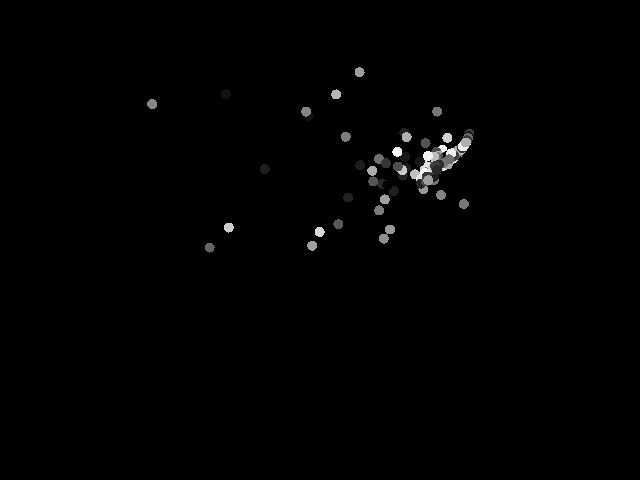
\includegraphics[width = 1\textwidth]{imgs/prace-s-objekty-1.png}
\end{center}

Rozeberme si jen letmo k čemu vlastně došlo. Nejprve jsme definovali prázdné pole určené pro naše entity. Posléze jsme mu stanovili velikost a celé pole jsme naplnili novými objekty entit  (odborněji instancemi). V poli se tedy nachází na každém místě pole jedna entita. Každou entitu poté ve funkci \vyraz{draw()} probouzíme k životu pomocí spuštění příkazu přes {\em tečkovou syntaxi} k posunu směrem ke kurzoru (funkcí {\em posunSeKeKurzoru()}) a následovnému vykreslení elipsy (funkcí {\em kresli()}).



\oddil{Náhoda}

V minulé kapitole jsme hovořili o výrazu \vyraz{random()}, nyní se pokusíme poodhalit tajemství náhody v programování.

Proč má smysl v případě strojů vůbec hovořit o náhodě. Náhoda je z pohledu výpočetní techniky třeba vnímat jako vnější vliv. V rámci počítačové logiky náhoda v podstatě neexistuje. Každý jev má svoji příčinu a může mít svůj následek. Počítačové jazyky znají jen pojem takzvané pseudonáhodnosti.

Předložka pseudo, již nastiňuje určitou náhražku. Pseudonáhodnost je ve své podstatě strojová simulace náhody v čistě logickém prostředí. Náhodou pojmenováváme zpravidla jev, který nedokážeme pro jeho složitost předpovědět. Reálný svět vnímaný člověkem obsahuje takzvanou pravou náhodu, tedy to, co skutečně nelze vypozorovat.

Situace přenesení náhody do světa logického uvažování je velmi problematická proto, že člověku se velmi těžko stroji popisuje fakt srozumitelnosti. Některé jednoduché pravidla srozumitelné jsou, jiné z pohledu výpočtu podobně jednoduché již ne.

Pseudonáhodou člověk definuje takový výpočet, který samozřejmě vychází z logického výpočtu, člověk jej již ovšem nedokáže předpovědět.

Konkrétní příklad jak lze v Processingu vygenerovat pseudonáhodné pomocí příkazu \vyraz{random()} číslo je:

\begin{lstlisting}
float nahodna = random(10);
println(nahoda);
\end{lstlisting}

Proměnná nazvaná nahoda nyní přijímá pseudonáhodnou hodnotu od nuly do deseti jež následovně vytiskne do konzole. Druhý možný zápis je zadání dvou čísel tedy rozsahu výsledné pseudonáhodné hodnoty.


\begin{lstlisting}
float nahodna = random(10,20);
println(nahoda);
\end{lstlisting}

Jak je zřejmě pochopitelné náhoda se nyní bude pohybovat v rozmezí čísla od deseti do dvaceti. To co se vám konkrétně objeví v konzoli nedokážu předpovědět, jedná se totiž o vaše náhodné číslo.

Tisk do konzole je samozřejmě jeden z možných výstupů. Náhodné číslo můžeme zobrazit graficky. Můžeme například animovat pozici elipsy na ploše:

\begin{lstlisting}
void setup(){
	size(640,480);
}


void draw(){
	background(255);
	fill(255);
	ellipse(width/2 + random(-5,5), height/2 + random(-5,5), 20, 20);
}
\end{lstlisting}


Spustíme-li tento program, uvidíme kmitající elipsu na středu kreslícího plátna. Kmitání probíhá v rozmezí od mínus pěti do plus pěti pixelů od středu v obou osách. Každé jednotlivé okénko se obměňuje nová pseudonáhodná hodnota, a tím dochází k animaci.


\pododdil{Šum}

Další možným strůjcem náhodně generované hodnoty je takzvaný Perlnův šum (Perlin noise). Perlinův šum je pojmenovaný po svém vynálezci Kenu Perlinovi a je velmi často využíván při generování přírodně vypadajícího náhodného pohybu. Oproti příkazu \vyraz{random()} se perlinův šum \vyraz{noise()} odvíjí plynule. Pro ilustraci si de můžeme ukázat rodíl mezi perlinovým šumem a holým pseudonáhodným číslem.

\begin{lstlisting}
void setup(){
	size(640,480);
}


void draw(){
	background(255);
	fill(255);
	ellipse(width/2 + noise( frameCount/30.0 ), height/2 + noise( frameCount/10.0 ), 20, 20);
}
\end{lstlisting}

Pohyb obrazce bude nyní probíhat plynule v nepředpovídatelných směrech. Příkaz \vyraz{noise()} předpokládá vstup, který určuje pozici v šumu. Perlinův šum si můžeme představit jako neměnný graf kterým můžeme procházet tam i zpět, v závislosti na zaslané hodnotě. Jelikož do příkazy \vyraz{noise()} posíláme proměnnou hodnotu \vyraz{frameCount} procházíme variacemi perlinova šumu, výstupem bude vždy číslo v rozmezí nula až jedna. Budeme-li potřebovat rozmezí jiné můžeme šum vynásobit požadovaným rozsahem (jak je tomu v předchozím příkladě).








\chapter{Práce s daty}


Jak jsme si v úvodu knihy \odkaz{Sketch} zmínili, adresář pro externí soubory se nazývá DATA. Tento adresář je umístěný přímo v adresáři projektu. Veškeré soubory, které do tohoto adresáře umístíme budou programu dostupné.

V případě ukládání bude Processing zapisovat relativně do adresáře projektu.

Ukažme si nyní jakým způsobem můžeme uložit a načíst vnější data do našeho programu.





\oddil{Ukládání informací}

Kresba do okna programu je jen jeden způsob výstupu programu. V určitém momentu budeme potřebovat zaznamenat obraz nebo jiná data pro další práci nebo archivaci. Processing umí ukládat data do razmanitých formátů, při práci s obrazem se jedná o základní druhy bitmap a vektorového výstupu ve standartizovaném formátu pdf.

Při ukládání holých dat můžeme například využít prosté textové soubory, které se hodí při dalším zpracování pomocí Processingu. Velmi častý formát takového zápisu je takzavný \slovnik{CSV}, což je v podstatě textový soubor obsahující data oddělená čárkou. Jeho velikost závisí na objemu dat. V případě hieraticky strukturovaných dat lze k uložení hearitcky uposřádaný formát XML.


\pododdil{Ukládání obrazových dat}

Doposud jsme pracovali s obrazem, který je dočasný. Po zavření okna Processingu obraz nenávratně zmizí. K tomu abychom z Processingu dostali obrazový výstup, potřebujeme kresbu uložit do souboru.

Processing umí ukládat různé formáty soubourů. Nejběžněji budeme potřebovat uložit obrazová data jako rastrový obrázek. Formát obrázku si můžeme zvolit.

Processing umí ukládat rastrová data do následujících formátů:


\begin{itemize}
\item
TIFF – nekomprimovaný obraz s příponou *.tif, *.tiff
\item
TARGA – ztrátově komprimovaný obraz s příponou *.tga
\item
JPEG – ztrátově komprimovaný obraz s příponou *.jpg
\item
PNG – bezztrátově komprimovaný obraz s příponou *.png

\end{itemize}

S některými formáty jste se již mohli setkat v minulosti. Jedná se o standartní a rozšířené formáty pro uchovávání obrazových dat.

Uložení obrázku ze současného plátna se provádí příkazem \slovnik{save()}. Příkaz potřebuje znát cestu a koncovku souboru. Nenapíšeme-li plnou cestu Processing data uloží přímo do naší sketche.

Nevíte-li kterou koncovku soboru zvolit, doporučil bych vám vřele formát PNG. Takzvaný Portable Network Graphics je standart, který vyniká relativně malou velikostí a bezztrátovou kompresí dat. Vaše data tak budou uložena jedna k jedné a můžete s nimi beze ztráty dále operovat. 

Samotné ukládání se provádí následujícím způsobem:

\begin{lstlisting} 
void setup(){
	size(640,480);
}

void draw(){
	background(255);
	line(mouseX,mouseY,pmouseX,pmouseY);

}

void mousePressed(){
	save("obrazek.png");
}

\end{lstlisting}


Příkaz \vyraz{save()} provede uložení obrazových dat okamžitě. Kdybychom vložili příkaz do kreslící smyčky Processing by se pokusil ukládat obrázek šedesátkrát za vteřinu, což by se mu z důvodů relativní náročnosti operace zřejmně nepodařilo a byli bychom svědky zpomalení rychlosti ve vykreslování.

V příkladě tedy budeme ukládat obrázek jen po kliknutí myší.





Nyní si představme, že z nějakého důvodu potřebujeme zachytit plnou sekvenci po sobě jdoucích obrázků. Problém příkazu save() je ten, že v případě natrvdo zadané cesty bude stále přepisovat obrazovými daty tentýž soubor. Abychom uložili vícero obrázků potřebujeme proměňovat cestu kam Processing obrázky ukládá. Můžeme k tomu využít počítadlo nebo zvláštní příkaz processingu \vyraz{saveFrame()};

\begin{lstlisting} 
void setup(){
	size(640,480);
}

void draw(){
	// kresba probehne zde

	save("obrazek" + nf( frameCount , 5 ) + ".png");
}

\end{lstlisting}

Využití počítadle je možné, ale trochu zdlouhavé. Všimněte si zde pouze způsobu jakým číslujeme názvy souborů. Hodnota \vyraz{frameCount} se mění podle počtu vykreslených okének. Příkaz \vyraz{nf()} je zde z kosmetických důvodů, přidává pouze daný počet nul před naše počítadlo. Celý tento zápis se se dá ovšem elegantně zkrátit příkazem \vyraz{saveFrame()}.


\begin{lstlisting} 
void setup(){
	size(640,480);
}

void draw(){
	// kresba probehne zde

	saveFrame("obrazek#####.png");
}

\end{lstlisting}

Příkaz \vyraz{saveFrame()} vyžaduje stejně jako příkaz \vyraz{save()} cestu k ukládanému souboru. Příkaz má ovšem navíc tu vlastnost, vložíme-li do názvu souboru znaky křížku, Processing je rozpozná jako počet nul v počítadle okének.



\pododdil{Ukládání holých dat}

Ukládání informací do obrazu je jen pouze jedna z možností. Někdy se nám může hodit uložit informace v jiném formátu. Řekněme že potřebujeme uložit pozice myši pro pozdejší animaci. Jistě bychom mohli uložit tuto informaci do série obrázků, z hlediska programování by to ovšem nebylo velmi prozřetelné.

Konkrétní údaje o pohybu kurzoru známe. Můžeme je tedy zaznamenat například do nám již známého pole souřadnic. Pro tento účel si vytvoříme program, který bude umět zaznamenávat údaje o pohybu kurzoru do textového souboru. Předtím než se pustíme do práce je dobré si uvědomit že text neobsahuje číselné informace. Vzpomínáte na kapitolu o základních datatypech? \odkaz{Základní datatypy} S textem, tedy ani potažmo textovým souborem, nelze manipulovat jako s čísly.

Při ukládání dat do textové podoby tedy musíme mít již na mysli jak je posléze budeme číst a proto zvolíme vhodný formát pro ukládání. Vhodným formátem pro uchovávání informací v textové podobě je takzvaný \slovnik{CSV}, comma separated value. Jak z anglického názvu vyplývá jedná se o hodnoty, které jsou oddělené čárkou. Pro naše potřeby budou stačit hodnoty dvě pro osu X a osu Y našeho kurzoru.

Program si můžeme navrhnout následovně:

\begin{lstlisting}
float osaX[];
float osaY[];
int pocetHodnot = 300;

void setup(){

	size(640,480);
	osaX = new float[pocetHodnot];
	osaY = new float[pocetHodnot];
}


void draw(){

	osaX[frameCount] = mouseX;
	osaY[frameCount] = mouseY;

	if(frameCount >= pocetHodnot-1){
		ulozDoSouboru();
		exit();
	}
}

void ulozDoSouboru(){

	String[] holyText = new String[pocetHodnot];
	for(int i = 0 ; i < pocetHodnot; i++){
		holyText[i] = osaX[i]+", "+osaY[i];
	}
	
	saveStrings("soubor.csv",holyText);
}
\end{lstlisting}

Program je hotový. Rozeberme si doposud nevídané věci. Pole by nám měla být již srozumitelná, v tomto případě pouze používáme datatyp \vyraz{float}. Vytvořili jsme si dvě rozdílná pole pro dvě osy.

 Ve funkci \vyraz{draw()} nyní dochází k samotnému zápisu, a to pomocí již známé proměnné \vyraz{frameCount()}. Pokaždé je hodnota zapsána na novou pozici. Následuje podmínka, která dříve novým příkazem \vyraz{exit()} ukončuje program. Podmínka je spuštěna pouze tehdy, máme-li již dostatečný počet zaznamenaných hodnot.
 
Podmínka navíc, předtím než ukončí celý program, spustí námi definovanou funkci pro uložení nashromážděných dat.

Tato funkce za pomoci smyčky převede číselné informace do textové podoby. Proměnné {\em osaX} a {\em osaY} funkce spojí dohromady pomocí znaménka plus spolu s čárkou a mezerou. Dále již následuje funkce Processingu \vyraz{saveStrings()}, která zajištuje zápis pole textu do souboru. Koncovku jsem zde zvolil {\em *.csv}, ale je možné použít jakoukoli jinou, např. {\em *.txt}.

 Podívejme se nyní do adresáře projektu. (pomocí klávesy \klavesy{CTRL + k}). Soubor s názvem {\em soubor.csv} by měl být plný zaznamenaných hodnot.
 
 
 \begin{center}
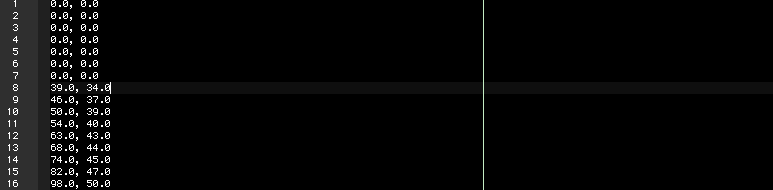
\includegraphics[width = 1\textwidth]{imgs/csv.png}
\end{center}

\pododdil{Tisk do pdf, ukládání vektorů}


\oddil{Načítání informací}

\pododdil{Načítání obrázků}
\pododdil{Načítání textových souborů}


\oddil{Pokročilejší operace se String}
\pododdil{Parsing, získávání hodnot z externích dat}

\chapter{Vizualizace hodnot}

\chapter{Rozšíření Processingu}
\oddil{Knihovny}

\pododdil{Vestavěné knihovny}
\index{vestavěné knihovny}

Ve skecthbooku se dále nacházejí\footnote{od verze 1.0} veškeré rozšíření za pomocí takzvaných knihoven neboli libraries. Ty jsou umístěny v adresáři sketchbooku ve složce {\em libraries}. Knihovny jsou silným rozšířením celého jazyka a pokrývají mnoho možností s nakládaáním s externími daty, zajišťují komunikaci zařízeními, práci s videem, zvukem, nebo s trojdimenzionálními daty či vektorovým obrazem.


Knihovny jsou v podstatě moduly které se zaměřují většinou na jeden problém. Některé moduly umí například komunikovat s kamerou, jiné umí přenášet informace přes síť nebo komunikovat se zařízeními. Knihovna je sada příkazů, která rozšiřuje samotný jazyk o nové možnosti.


Knihovnami se také dá dobře ilustrovat k čemu uživatelé Processingu převážně programovací prostředí využívají. To sice nemusí být v žádném případě směrodatné pro vaší práci, může to být ovšem i velmi inspirativní. Knihovny Vám pomohou získat jistý přehled o kontextu užívání Processingu.

Knihovny se  nejobecněji dělí na dvě základní skupiny. Jednu tvoří interní knihovny Processingu, které přichází již nainstalované se softwarem a knihovny vější, vytvořené komunitou uživatelů. Veškeré nainstalovaná knihovny, které má Processing k dispozici, lze nalézt pod tlačítkem sketch > Import Library.


Výčet komunitnách knihoven je již poměrné obsáhlý, pro ilustraci zde budeme hovořit jen o knihovnách vestavěných. Věstavěných knihoven je nepoměrně méně, jejich výčet se proměňuje relativně pomalu, jejich dokumentace je kvalitně zpracovaná:


\begin{itemize}
\item
Video

Základní rozhraní mezi Apple Qucktime a Processingem. U platformy Linux, tato knihovna dlouhodobě nefunguje kvůli závislosti na propietárním softwaru, musíme tedy využít alternativy. Například implementace nativní knihovny GStreamer.

\item
Network
Zajišťuje základní síťovou + internetovou komunikaci. 

\item
Serial
Podpora pro komunikaci se sériovými porty, externí zařízeni typu (RS-232).

\item
PDF Export
Knihovna pro export do PDF.

\item
OpenGL
Technologie pro podporu java implementace akcelerované grafiky JOGL.

\item
Minim
Využívá JavaSound API ke snadné obsluze zvukového výstupu.

\item
DXF Export
Knihovna pro exportování vektorových dat ve formátu DXF (Autocad, 3D).

\item
Arduino
Knihovna určená pro komunikaci s Arduinem.

\item
Netscape.JavaScript
Nese metody pro komunikaci s Javascriptem a Processingovým appletem ve své webové podobě.

\item
Candy SVG Import
Knihovna pro načítání vektorové grafiky ve formátu SVG (Inkscape, Adobe Illustrator)

\item
XML Import
Podpora načítání XML tabulek.
\end{itemize}

Neříkají-li vám tyto zkratky nic, nevadí, jedná se většinou o datové standarty a typy zařízení se kterými můžete s pomocí knihoven pracovat. Každá z těchto knihoven má svoji dobrou dokumentaci na stránkách projektu, nebo přímo v tzv. {\em Examples}, příkladech pro každou knihovnu, lze tímto způsobem zobrazit základní nápovědu.


\oddil{Nástroje}
.
\newpage
\oddil{Komplexní program}
.
\newpage
\oddil{Experimenty}


\chapter{Rejstřík pojmů}
\printglossaries
\printindex


%\printindex



\end{document}
